% Options for packages loaded elsewhere
\PassOptionsToPackage{unicode}{hyperref}
\PassOptionsToPackage{hyphens}{url}
\hyphenpenalty=10000
%
\documentclass[
  12pt,
  a4paperpaper,
]{report}
\usepackage{lmodern}
\usepackage{amssymb,amsmath}
\usepackage{ifxetex,ifluatex}
\ifnum 0\ifxetex 1\fi\ifluatex 1\fi=0 % if pdftex
  \usepackage[T1]{fontenc}
  \usepackage[utf8]{inputenc}
  \usepackage{textcomp} % provide euro and other symbols
\else % if luatex or xetex
  \usepackage{unicode-math}
  \defaultfontfeatures{Scale=MatchLowercase}
  \defaultfontfeatures[\rmfamily]{Ligatures=TeX,Scale=1}
\fi
% Use upquote if available, for straight quotes in verbatim environments
\IfFileExists{upquote.sty}{\usepackage{upquote}}{}
\IfFileExists{microtype.sty}{% use microtype if available
  \usepackage[]{microtype}
  \UseMicrotypeSet[protrusion]{basicmath} % disable protrusion for tt fonts
}{}
\makeatletter
\@ifundefined{KOMAClassName}{% if non-KOMA class
  \IfFileExists{parskip.sty}{%
    \usepackage{parskip}
  }{% else
    \setlength{\parindent}{0pt}
    \setlength{\parskip}{6pt plus 2pt minus 1pt}}
}{% if KOMA class
  \KOMAoptions{parskip=half}}
\makeatother
\usepackage{xcolor}
\IfFileExists{xurl.sty}{\usepackage{xurl}}{} % add URL line breaks if available
\IfFileExists{bookmark.sty}{\usepackage{bookmark}}{\usepackage{hyperref}}
\hypersetup{
  hidelinks,
  pdfcreator={LaTeX via pandoc}}
\urlstyle{same} % disable monospaced font for URLs
\usepackage{color}
\usepackage{fancyvrb}
\newcommand{\VerbBar}{|}
\newcommand{\VERB}{\Verb[commandchars=\\\{\}]}
\DefineVerbatimEnvironment{Highlighting}{Verbatim}{commandchars=\\\{\}}
% Add ',fontsize=\small' for more characters per line
\newenvironment{Shaded}{}{}
\newcommand{\AlertTok}[1]{\textcolor[rgb]{1.00,0.00,0.00}{\textbf{#1}}}
\newcommand{\AnnotationTok}[1]{\textcolor[rgb]{0.38,0.63,0.69}{\textbf{\textit{#1}}}}
\newcommand{\AttributeTok}[1]{\textcolor[rgb]{0.49,0.56,0.16}{#1}}
\newcommand{\BaseNTok}[1]{\textcolor[rgb]{0.25,0.63,0.44}{#1}}
\newcommand{\BuiltInTok}[1]{#1}
\newcommand{\CharTok}[1]{\textcolor[rgb]{0.25,0.44,0.63}{#1}}
\newcommand{\CommentTok}[1]{\textcolor[rgb]{0.38,0.63,0.69}{\textit{#1}}}
\newcommand{\CommentVarTok}[1]{\textcolor[rgb]{0.38,0.63,0.69}{\textbf{\textit{#1}}}}
\newcommand{\ConstantTok}[1]{\textcolor[rgb]{0.53,0.00,0.00}{#1}}
\newcommand{\ControlFlowTok}[1]{\textcolor[rgb]{0.00,0.44,0.13}{\textbf{#1}}}
\newcommand{\DataTypeTok}[1]{\textcolor[rgb]{0.56,0.13,0.00}{#1}}
\newcommand{\DecValTok}[1]{\textcolor[rgb]{0.25,0.63,0.44}{#1}}
\newcommand{\DocumentationTok}[1]{\textcolor[rgb]{0.73,0.13,0.13}{\textit{#1}}}
\newcommand{\ErrorTok}[1]{\textcolor[rgb]{1.00,0.00,0.00}{\textbf{#1}}}
\newcommand{\ExtensionTok}[1]{#1}
\newcommand{\FloatTok}[1]{\textcolor[rgb]{0.25,0.63,0.44}{#1}}
\newcommand{\FunctionTok}[1]{\textcolor[rgb]{0.02,0.16,0.49}{#1}}
\newcommand{\ImportTok}[1]{#1}
\newcommand{\InformationTok}[1]{\textcolor[rgb]{0.38,0.63,0.69}{\textbf{\textit{#1}}}}
\newcommand{\KeywordTok}[1]{\textcolor[rgb]{0.00,0.44,0.13}{\textbf{#1}}}
\newcommand{\NormalTok}[1]{#1}
\newcommand{\OperatorTok}[1]{\textcolor[rgb]{0.40,0.40,0.40}{#1}}
\newcommand{\OtherTok}[1]{\textcolor[rgb]{0.00,0.44,0.13}{#1}}
\newcommand{\PreprocessorTok}[1]{\textcolor[rgb]{0.74,0.48,0.00}{#1}}
\newcommand{\RegionMarkerTok}[1]{#1}
\newcommand{\SpecialCharTok}[1]{\textcolor[rgb]{0.25,0.44,0.63}{#1}}
\newcommand{\SpecialStringTok}[1]{\textcolor[rgb]{0.73,0.40,0.53}{#1}}
\newcommand{\StringTok}[1]{\textcolor[rgb]{0.25,0.44,0.63}{#1}}
\newcommand{\VariableTok}[1]{\textcolor[rgb]{0.10,0.09,0.49}{#1}}
\newcommand{\VerbatimStringTok}[1]{\textcolor[rgb]{0.25,0.44,0.63}{#1}}
\newcommand{\WarningTok}[1]{\textcolor[rgb]{0.38,0.63,0.69}{\textbf{\textit{#1}}}}
\usepackage{longtable,booktabs}
% Correct order of tables after \paragraph or \subparagraph
\usepackage{etoolbox}
\makeatletter
\patchcmd\longtable{\par}{\if@noskipsec\mbox{}\fi\par}{}{}
\makeatother
% Allow footnotes in longtable head/foot
\IfFileExists{footnotehyper.sty}{\usepackage{footnotehyper}}{\usepackage{footnote}}
\makesavenoteenv{longtable}
\usepackage{graphicx,grffile}
\makeatletter
\def\maxwidth{\ifdim\Gin@nat@width>\linewidth\linewidth\else\Gin@nat@width\fi}
\def\maxheight{\ifdim\Gin@nat@height>\textheight\textheight\else\Gin@nat@height\fi}
\makeatother
% Scale images if necessary, so that they will not overflow the page
% margins by default, and it is still possible to overwrite the defaults
% using explicit options in \includegraphics[width, height, ...]{}
\setkeys{Gin}{width=\maxwidth,height=\maxheight,keepaspectratio}
% Set default figure placement to htbp
\makeatletter
\def\fps@figure{htbp}
\makeatother
\setlength{\emergencystretch}{3em} % prevent overfull lines
\providecommand{\tightlist}{%
  \setlength{\itemsep}{0pt}\setlength{\parskip}{0pt}}
\setcounter{secnumdepth}{5}


% Table of contents formatting
\renewcommand{\contentsname}{Table of Contents}
\setcounter{tocdepth}{3}

% Headers and page numbering
\usepackage{fancyhdr}
\pagestyle{plain}

\usepackage{algorithm2e}
% Following package is used to add background image to front page
\usepackage{wallpaper}

% Table package
\usepackage{ctable}% http://ctan.org/pkg/ctable

% Deal with 'LaTeX Error: Too many unprocessed floats.'
\usepackage{morefloats}
% or use \extrafloats{100}
% add some \clearpage

% % Chapter header
% \usepackage{titlesec, blindtext, color}
% \definecolor{gray75}{gray}{0.75}
% \newcommand{\hsp}{\hspace{20pt}}
% \titleformat{\chapter}[hang]{\Huge\bfseries}{\thechapter\hsp\textcolor{gray75}{|}\hsp}{0pt}{\Huge\bfseries}

% % Fonts and typesetting
% \setmainfont[Scale=1.1]{Helvetica}
% \setsansfont[Scale=1.1]{Verdana}

% FONTS
\usepackage{xunicode}
\usepackage{xltxtra}
\defaultfontfeatures{Mapping=tex-text} % converts LaTeX specials (``quotes'' --- dashes etc.) to unicode
% \setromanfont[Scale=1.01,Ligatures={Common},Numbers={OldStyle}]{Palatino}
% \setromanfont[Scale=1.01,Ligatures={Common},Numbers={OldStyle}]{Adobe Caslon Pro}
%Following line controls size of code chunks
% \setmonofont[Scale=0.9]{Monaco}
%Following line controls size of figure legends
% \setsansfont[Scale=1.2]{Optima Regular}

% CODE BLOCKS
\usepackage[utf8]{inputenc}
\usepackage{listings}
\usepackage{color}

% JAVA CODE BLOCKS
\definecolor{backcolour}{RGB}{242,242,242}
\definecolor{javared}{rgb}{0.6,0,0}
\definecolor{javagreen}{rgb}{0.25,0.5,0.35}
\definecolor{javapurple}{rgb}{0.5,0,0.35}
\definecolor{javadocblue}{rgb}{0.25,0.35,0.75}

\lstdefinestyle{javaCodeStyle}{
  language=Java,                         % the language of the code
  backgroundcolor=\color{backcolour},    % choose the background color; you must add \usepackage{color} or \usepackage{xcolor}
  basicstyle=\fontsize{10}{8}\sffamily,
  breakatwhitespace=false,
  breaklines=true,
  keywordstyle=\color{javapurple}\bfseries,
  stringstyle=\color{javared},
  commentstyle=\color{javagreen},
  morecomment=[s][\color{javadocblue}]{/**}{*/},
  captionpos=t,                          % sets the caption-position to bottom
  frame=single,                          % adds a frame around the code
  numbers=left,
  numbersep=10pt,                         % margin between number and code block
  keepspaces=true,                       % keeps spaces in text, useful for keeping indentation of code (possibly needs columns=flexible)
  columns=fullflexible,
  showspaces=false,                      % show spaces everywhere adding particular underscores; it overrides 'showstringspaces'
  showstringspaces=false,                % underline spaces within strings only
  showtabs=false,                        % show tabs within strings adding particular underscores
  tabsize=2                              % sets default tabsize to 2 spaces
}

%Attempt to set math size
%First size must match the text size in the document or command will not work
%\DeclareMathSizes{display size}{text size}{script size}{scriptscript size}.
\DeclareMathSizes{12}{13}{7}{7}

% ---- CUSTOM AMPERSAND
% \newcommand{\amper}{{\fontspec[Scale=.95]{Adobe Caslon Pro}\selectfont\itshape\&}}

% HEADINGS
\usepackage{sectsty}
\usepackage[normalem]{ulem}
\sectionfont{\rmfamily\mdseries\Large}
\subsectionfont{\rmfamily\mdseries\scshape\large}
\subsubsectionfont{\rmfamily\bfseries\upshape\large}
% \sectionfont{\rmfamily\mdseries\Large}
% \subsectionfont{\rmfamily\mdseries\scshape\normalsize}
% \subsubsectionfont{\rmfamily\bfseries\upshape\normalsize}

% Set figure legends and captions to be smaller sized sans serif font
\usepackage[font={footnotesize,sf}]{caption}

\usepackage{siunitx}

% Adjust spacing between lines to 1.5
\usepackage{setspace}
\onehalfspacing
% \doublespacing
\raggedbottom

% Set margins
\usepackage[top=1.5in,bottom=1.5in,left=1.5in,right=1.4in]{geometry}
% \setlength\parindent{0.4in} % indent at start of paragraphs (set to 0.3?)
\setlength{\parskip}{9pt}

% Add space between pararaphs
% http://texblog.org/2012/11/07/correctly-typesetting-paragraphs-in-latex/
% \usepackage{parskip}
% \setlength{\parskip}{\baselineskip}

% Set colour of links to black so that they don't show up when printed
\usepackage{hyperref}
\hypersetup{colorlinks=false, linkcolor=black}

% Tables
\usepackage{booktabs}
\usepackage{threeparttable}
\usepackage{array}
\newcolumntype{x}[1]{%
>{\centering\arraybackslash}m{#1}}%

% Allow for long captions and float captions on opposite page of figures
% \usepackage[rightFloats, CaptionBefore]{fltpage}

% Don't let floats cross subsections
% \usepackage[section,subsection]{extraplaceins}

\date{}

\begin{document}

\begin{titlepage}
    \begin{center}

    % Delete the following line
    % to remove the UCL header logo
    %\ThisULCornerWallPaper{1.0}{style/univ_logo.eps}
        
        \vspace*{2.5cm}
        
        \huge
        AMALTHEA-based GPU Response Time Analysis for NVidia's Jetson TX2
        
        \vspace{1.5cm}
        
        \Large
        Daniel Leoncio Paredes Zevallos 

        \vspace{1.5cm}

        \normalsize
        A thesis presented for the degree of\\
        Master of Engineering
        
        \vfill
        
        \normalsize
        Supervised by:\\
        Professor Dr. Carsten Wolff\\
        Herr Robert Hoettger

        \vspace{0.8cm}

        % Uncomment the following line
        % to add a centered university logo
        % \includegraphics[width=0.4\textwidth]{style/univ_logo.eps}
        
        \normalsize
        Fachhochschule Dortmund, Germany\\
        October 2019

        % Except where otherwise noted, content in this thesis is licensed under a Creative Commons Attribution 4.0 License (http://creativecommons.org/licenses/by/4.0), which permits unrestricted use, distribution, and reproduction in any medium, provided the original work is properly cited. Copyright 2015,Tom Pollard.

    \end{center}
\end{titlepage}

\hypertarget{abstract}{%
\chapter*{Abstract}\label{abstract}}
\addcontentsline{toc}{chapter}{Abstract}

The purpose of the thesis is to calculate response times for
AMALTHEA-based models to analyze timing behaviors of CUDA kernels on
NVIDIA Jetson TX2's GPU. This work was focused on the context of the Bosch
WATERS Challenge 2019 {[}6{]}. The challenge focuses on timing-analysis for
heterogeneous software and hardware systems based on centralized end-to-end
architectures. The embedded platform NVIDIA Jetson TX2 was the selected platform for
testing. Furthermore, key concepts related to NVIDIA's GPU architecture
are presented, as well as a detailed explanation of rules behind
platform's GPU scheduler.
This work is based on these rules and experimental results show
the accuracy of our approach to estimate completion times for kernels
executed on Jetson TX2 platform. Experiments use real timing data from NVIDIA's
platform. Moreover, the algorithm is implemented in  Eclipse APP4MC, which allows an AMALTHEA-based response time analysis for NVIDIA's Jetson TX2.

\pagenumbering{roman}
\setcounter{page}{1}

\hypertarget{declaration-of-authorship}{%
\chapter*{Declaration of Authorship}\label{declaration-of-authorship}}
\addcontentsline{toc}{chapter}{Declaration of Authorship}

I hereby declare that the thesis submitted is my own unaided work. All
direct or indirect sources used are acknowledged as references. I am
aware that the thesis in digital form can be examined for the use of
unauthorized aid and in order to determine whether the thesis as a whole
or parts incorporated in it may be deemed as plagiarism. For the
comparison of my work with existing sources I agree that it shall be
entered in a data base where it shall also remain after examination, to
enable comparison with future theses submitted. Further rights of
reproduction and usage, however,are not granted here. This thesis was
not previously presented to another examination board and has not been
published.

Place and Date
\quad\quad\quad\quad\quad\quad\quad\quad\quad\quad\quad\quad\quad\quad Signature

\hypertarget{ehrenwuxf6rtliche-erkluxe4rung}{%
\chapter*{Ehrenwörtliche
Erklärung}\label{ehrenwuxf6rtliche-erkluxe4rung}}
\addcontentsline{toc}{chapter}{Ehrenwörtliche Erklärung}

Ich erkläre hiermit ehrenwörtlich, dass ich die vorliegende Arbeit
selbständig angefertigt habe. Die aus fremden Quellen direkt und
indirekt übernommenen Gedanken sind als solche kenntlich gemacht.Ich
weiß, dass die Arbeit in digitalisierter Form daraufhin überprüft werden
kann, ob unerlaubte Hilfsmittel verwendet wurden und ob es sich -
insgesamt oder in Teilen - um ein Plagiat handelt. Zum Vergleich einer
Arbeit mit existierenden Quellen darf sie in eine Datenbanke ingestellt
werden und nach der Überprüfung zum Vergleich mit künftige ingehenden
Arbeiten dort verbleiben. Weitere Vervielfältigungs- und
Verwertungsrechte werden dadurch nicht eingeräumt. Die Arbeit wurde
weder einer anderen Prüfungsbehörde vorgelegt noch veröffentlicht.

Ort, Datum
\quad\quad\quad\quad\quad\quad\quad\quad\quad\quad\quad\quad\quad\quad  Unterschrifft

\newpage

\pagenumbering{gobble}

\tableofcontents
\setcounter{tocdepth}{1}
\listoffigures
\listoftables

\newpage

\hypertarget{abbreviations-and-symbols}{%
\chapter*{Abbreviations and Symbols}\label{abbreviations-and-symbols}}
\addcontentsline{toc}{chapter}{Abbreviations and Symbols}

\hypertarget{abbreviations}{%
\section*{Abbreviations}\label{abbreviations}}
\addcontentsline{toc}{section}{Abbreviations}

\begin{tabbing}
\textbf{API}~~~~~~~~~~~~ \= \textbf{A}pplication \textbf{P}rogramming \textbf{I}nterface \\
\textbf{CE} \> \textbf{C}opy \textbf{E}ngine \\
\textbf{CPU} \> \textbf{C}entral \textbf{P}rocessing \textbf{U}nit \\
\textbf{EE} \> \textbf{E}xecution \textbf{E}ngine \\
\textbf{FIFO} \> \textbf{F}irst \textbf{I}n \textbf{F}irst \textbf{O}ut \\
\textbf{GPU} \> \textbf{G}raphics \textbf{P}rocessing \textbf{U}nit \\  
\textbf{HMP} \> \textbf{H}eterogeneous \textbf{M}ulti-\textbf{P}rocessor \\  
\textbf{SM} \> \textbf{S}treaming \textbf{M}ultiprocessor \\  
\textbf{OS} \> \textbf{O}perating \textbf{S}ystem \\
\end{tabbing}

\hypertarget{symbols}{%
\section*{Symbols}\label{symbols}}
\addcontentsline{toc}{section}{Symbols}

\begin{tabbing}
$\tau$~~~~~~~~~~~~ \= Set of tasks or kernels \\
$\tau_i$ \> Task or kernel $i$\\
$T_i$ \> Period of $\tau_i$ \\
$g_i$ \> Grid size of $\tau_i$ \\
$b_i$ \> Number of thread per block within $g_i$ \\
$C_i$ \> Execution time workload of a thread within $b_i$ \\
$u_i$ \> Utilization of $\tau_i$ \\
$r_i$ \> Release time of $\tau_i$ \\
$f_i$ \> Completion time of $\tau_i$ \\
$R_i$ \> Response time of $\tau_i$ \\
$U_t$ \> Total utilization of $\tau$ \\
$b_{max}$ \> Maximum amount of threads in a SM \\
$g_{max}$ \> Maximum amount of blocks that can be allocated in a SM \\
$g_f(t)$ \> Available blocks at  time t\\
$t_a$ \> Point in time at which a block will be allocated \\
\end{tabbing}

\newpage
\setcounter{page}{1}
\renewcommand{\thepage}{\arabic{page}}

\hypertarget{introduction}{%
\chapter{Introduction}\label{introduction}}

\hypertarget{motivation}{%
\section{Motivation}\label{motivation}}

Car manufactures want to reduce cost in terms of money and time required
to develop, test and validate a new piece of software and hardware due to a change of
supplier. For that reason, centralized end-to-end architectures are the
solution they are aiming to, because, for car companies such as BWW and
Audi, the car of future will be similar to a ``data center on wheels''
{[}1{]}.

Centralized end-to-end architectures would be the first step stone
towards decoupling software and hardware {[}2{]}. This type of
architectures will not only take advantage of internet connectivity,
cloud computing and powerful heterogeneous processing units, but also
allow scalable, hierarchical and highly integrated system.
In other words, car manufactures prefer low-latency,
hierarchical and cost effectiveness of centralized end-to-end
architectures, because of today's requirements of computational power,
bandwidth, integration, safety and real-time {[}3{]}.

However, car manufactures take into account that in centralized
end-to-end architectures different types of software would run on top
of an heterogeneous hardware supplied by companies such as NVIDIA,
Mobileye or Qualcomm. Thus, it is important to analyze and understand how
software behaves under those conditions, in order to ensure a
predictable and efficient system.

\hypertarget{industrial-challenge-waters-2019}{%
\section{Industrial challenge WATERS
2019}\label{industrial-challenge-waters-2019}}

Predictability is a key property for safety-critical and hard real-time
systems {[}4{]}. Analyzing time related characteristics is an important
step to design predictable embedded systems. However, in multi-core or
heterogeneous systems based on centralized end-to-end architectures it is
harder to satisfy timing constrains due to scheduling, caches,
pipelines and out-of-order executions {[}5{]}. 
Thus, development of timing-analysis methods for these types of
architectures has become, nowadays, one of the main focus of research in
both industry and academic environment.

Every year \emph{the WATERS Challenge} is announced.
The purpose of the WATERS industrial challenge is to
share ideas, experiences and solutions to concrete timing verification
problems issued from real industrial case studies {[}6{]}.

This year, 2019, the challenge focuses on timing-analysis for
heterogeneous software-hardware systems based on centralized end-to-end
architectures. The platform chosen for this purpose is the NVIDIA®
Jetson™ TX2 platform, which has a heterogeneous architecture equipped
with a Quad ARM A57 processor, a dual Denver processor, 8GB of LPDDR4
memory and 256 CUDA cores of NVIDIA's Pascal Architecture. 
An AMALTHEA model based on this platform is available {[}6{]}.
Developers can design solutions and test them later on real hardware.

\hypertarget{nvidia-jetson-tx2-architecture-overview}{%
\section{NVIDIA Jetson TX2: Architecture
Overview}\label{nvidia-jetson-tx2-architecture-overview}}

NVIDIA Jetson TX2 is an embedded system-on-module (SOM). It is ideal for
deploying advanced AI to remote field locations with poor or expensive
internet connectivity, robotics, gaming devices, Virtual Reality (VR),
Augmented Reality (AR) and portable medical devices. In addition, it
offers near-real-time responsiveness and minimal latency which is key for
intelligent machines that need mission-critical autonomy like mining{[}7{]}.

The main components of the Jetson TX2 are a dual-core ARMv8 based NVIDIA
Denver2, quad-core ARMv8 Cortex-A57, 8GB 128-bit LPDDR4 and integrated
256-core Pascal NVIDIA GPU. The quad-core Cortex-A57 and the dual-core
NVIDIA Denver2 can be seen as a cluster of heterogeneous multiprocessors
(HMP) {[}8{]}. Both HMP and GPU share a 8GB SRAM memory as shown in
Figure \ref{img:overview_arch}. Hereafter, whenever the term
\textbf{host} will refer to HMP, similarly  \textbf{device} will refer to GPU.

\begin{figure}
\centering
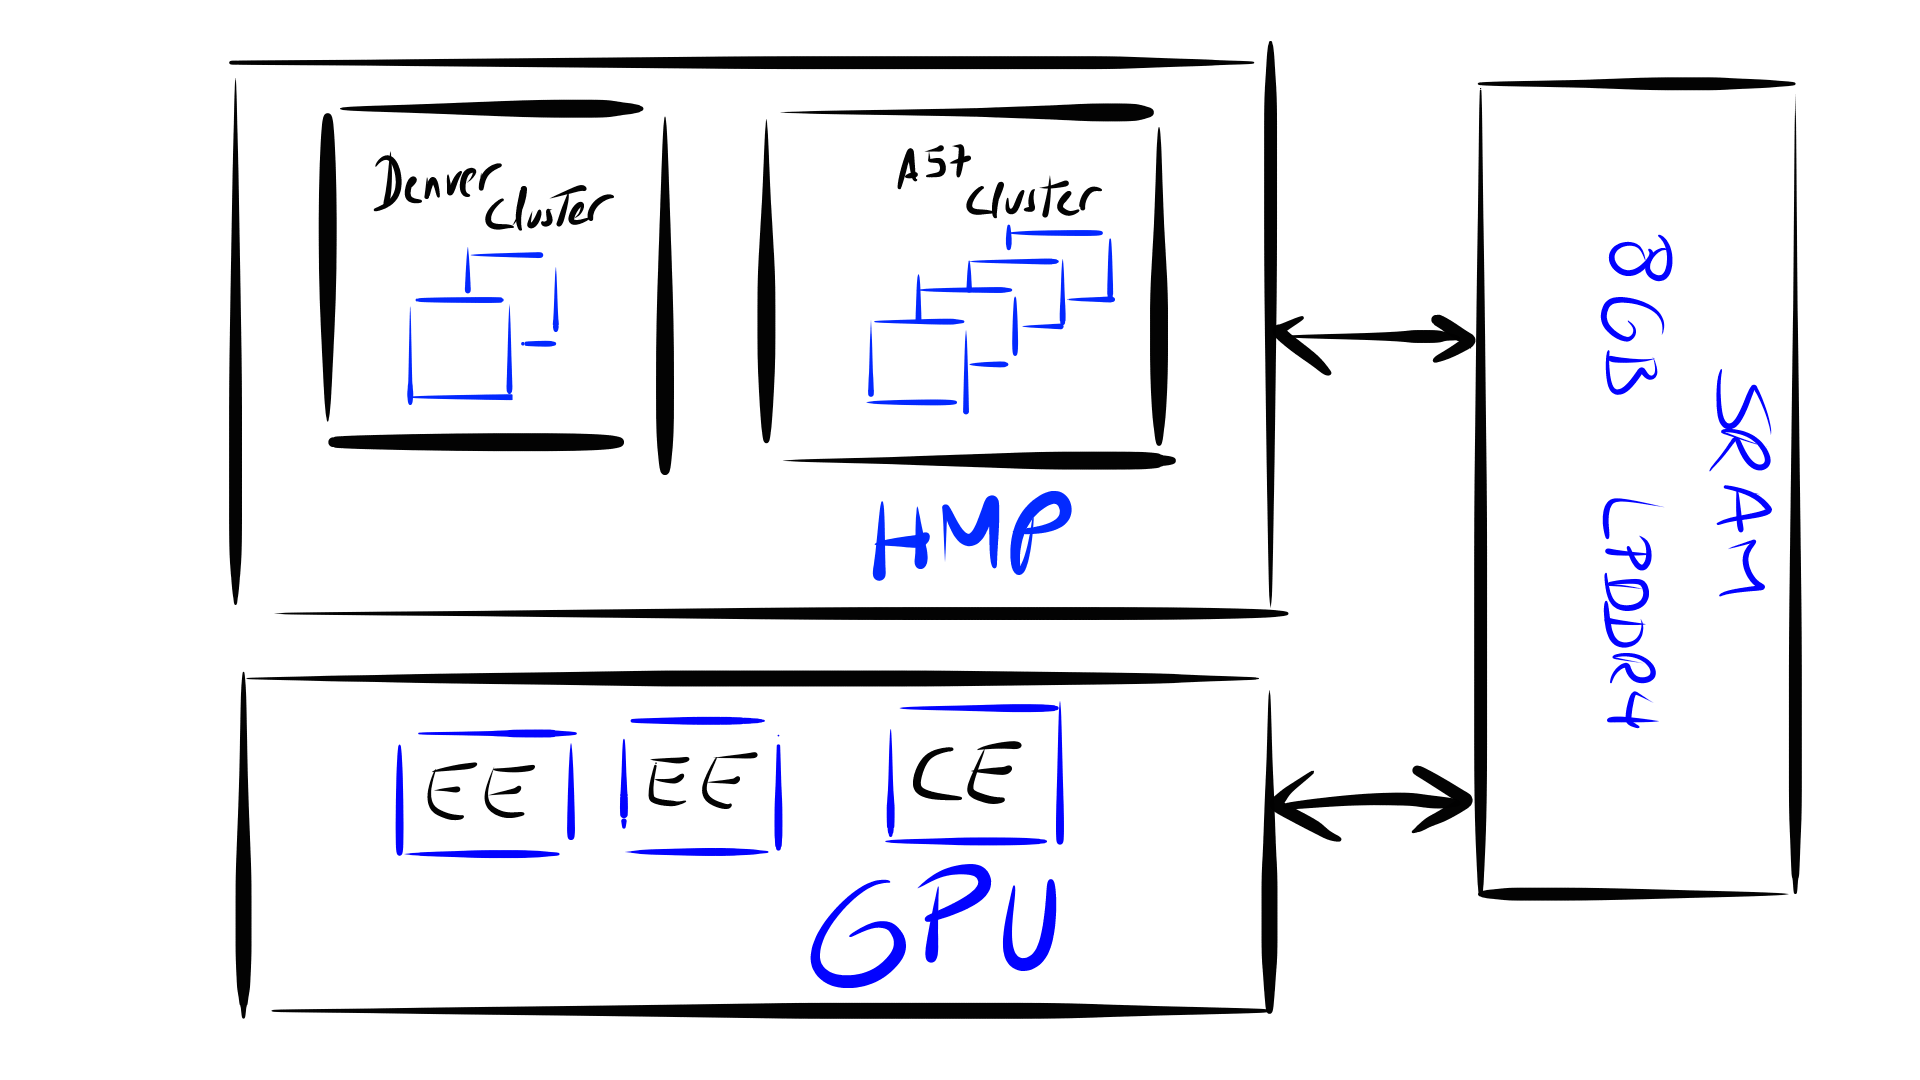
\includegraphics[width=1\textwidth,height=\textheight]{source/figures/overview_arch.png}
\caption{Jetson TX2 Architecture Overview \label{img:overview_arch}}
\end{figure}

Any NVIDIA GPU has two types of engines, \textbf{Copy Engines} (CE) and
\textbf{Execution Engines} (EE). The Jetson TX2 has only one CE and two
EE also known as \textbf{Streaming multiprocessors}. The CE is in charge of
data transfers from host to device and viceversa. There is, moreover,
the possibility that EE and CE run concurrently.

The GPU uses \textbf{streams} to run applications. The number of streams
depends on the GPU resources. An application can run in one or multiple
streams, the GPU scheduler, by default, manages how the application 
are allocated on streams in order to maximize throughput. In Chapter 2,
it is discussed how the TX2 GPU scheduler behaves in case
of multiple applications in more detail.

\hypertarget{jetson-tx2-amalthea-model}{%
\section{Jetson TX2 Amalthea Model}\label{jetson-tx2-amalthea-model}}

APP4MC is a platform for engineering multi- and many-core embedded
systems. This platform enables the creation and management of complex
tool chains including simulation and validation based on AMALTHEA models{[}9{]}.
In the context of the WATERS Challenge 2019, Bosch offers an AMALTHEA model of the Jetson TX2.
In this model, a CPU runnable reads data from memory, executes some computation (Ticks) and writes back data into memory as shown in Figure \ref{img:amalthea01}.

\begin{figure}
\centering
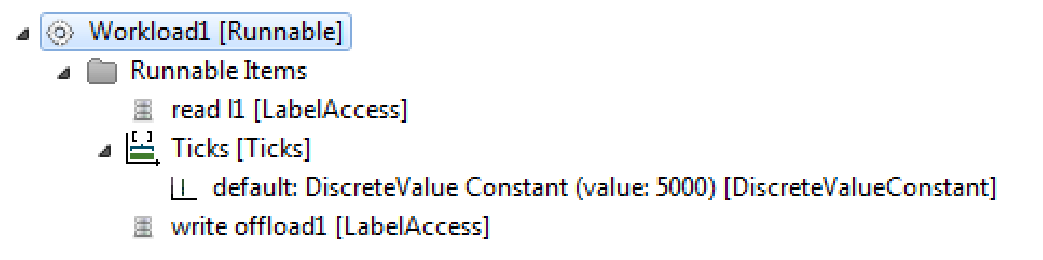
\includegraphics{source/figures/amalthea-01.png}
\caption{Runnable example for a CPU {[}6{]} \label{img:amalthea01}}
\end{figure}

In the case of GPU modeling, the runnable follows the same pattern
as in the CPU case: read, execution, write back. However, the reading
operation is actually to copy memory from host to device, thus it is
modeled as \emph{memory reading from host} and then as \emph{memory
writing to device}. On the other hand, the writing back operation
requires to copy memory from device to host therefore it is modeled as
\emph{memory reading from device} and then as \emph{memory writing to
host} as shown in Figure \ref{img:amalthea02}.

\begin{figure}
\centering
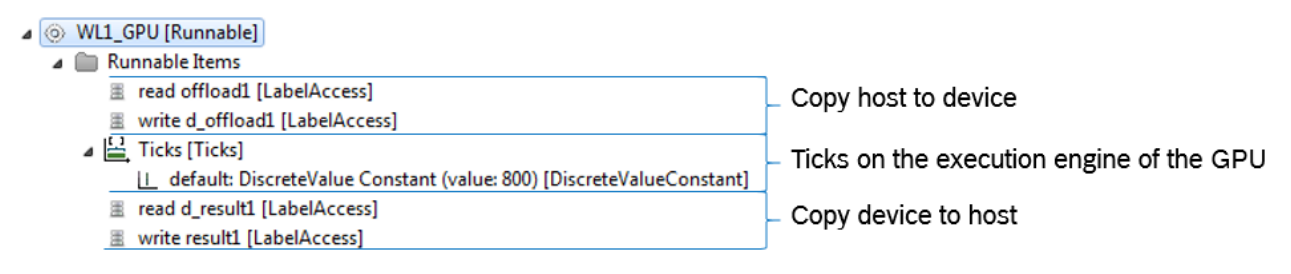
\includegraphics{source/figures/amalthea-02.png}
\caption{Runnable example for a GPU {[}6{]} \label{img:amalthea02}}
\end{figure}

\hypertarget{cuda-and-jetson-tx2}{%
\chapter{CUDA and Jetson TX2}\label{cuda-and-jetson-tx2}}

In this chapter an overview of the theorical background of
the NVIDIA GPU software and hardware model is given. 
There is also an introduction to the concepts of threads, blocks, kernels and streaming multriprocesor, and how they apply to this work's study case.
Jetson TX2's memory hierarchy and scheduler are presented in addition to the rules behind the Jetson TX2's hardware scheduler. At the end there is a comprehensive example.

\hypertarget{nvidia-gpu-software-model}{%
\section{NVIDIA GPU Software Model}\label{nvidia-gpu-software-model}}

Nowadays applications run on heterogeneous hardware and GPUs
are important in order to achieve high performance computing. Since 2006,
a running software on NVIDIA GPUs are known as a \emph{CUDA application}
{[}10{]}. A CUDA application runs concurrently multiple instances of
special functions called \textbf{kernels}. Each instance runs on a
\textbf{thread}. Moreover, these threads are arranged in
\textbf{blocks} and blocks compose \textbf{grids} as shown in Figure
\ref{img:sw_model_grids}.

\begin{figure}
\centering
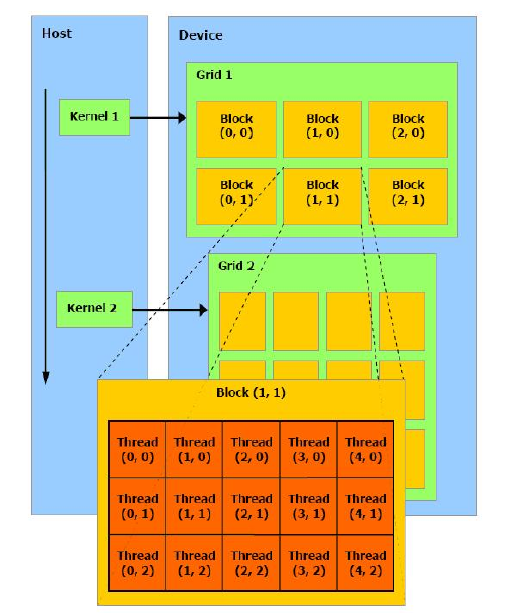
\includegraphics[width=0.6\textwidth,height=\textheight]{source/figures/sw_model_grids.png}
\caption{Organisation of grids, blocks, threads, and kernels {[}11{]}.
\label{img:sw_model_grids}}
\end{figure}

There is also a hierarchical memory
structure. Threads, blocks and grids have access to different memory
spaces as ilustrated in Figure \ref{img:sw_model_memory}. The types of
memory are summarized in Table \ref{tab:memory_hierarchy}.


\begin{longtable}[]{@{}llll@{}}
\caption{Types of memories in a GPU
\label{tab:memory_hierarchy}}\tabularnewline
\toprule
\begin{minipage}[b]{0.13\columnwidth}\raggedright
Memory\strut
\end{minipage} & \begin{minipage}[b]{0.53\columnwidth}\raggedright
Main Characteristics\strut
\end{minipage} & \begin{minipage}[b]{0.09\columnwidth}\raggedright
Scope\strut
\end{minipage} & \begin{minipage}[b]{0.13\columnwidth}\raggedright
Lifetime\strut
\end{minipage}\tabularnewline
\midrule
\endfirsthead
\toprule
\begin{minipage}[b]{0.13\columnwidth}\raggedright
Memory\strut
\end{minipage} & \begin{minipage}[b]{0.53\columnwidth}\raggedright
Main Characteristics\strut
\end{minipage} & \begin{minipage}[b]{0.09\columnwidth}\raggedright
Scope\strut
\end{minipage} & \begin{minipage}[b]{0.13\columnwidth}\raggedright
Lifetime\strut
\end{minipage}\tabularnewline
\midrule
\endhead
\begin{minipage}[t]{0.13\columnwidth}\raggedright
Global\strut
\end{minipage} & \begin{minipage}[t]{0.53\columnwidth}\raggedright
R/W, Slow and big\strut
\end{minipage} & \begin{minipage}[t]{0.09\columnwidth}\raggedright
Grid\strut
\end{minipage} & \begin{minipage}[t]{0.13\columnwidth}\raggedright
Application\strut
\end{minipage}\tabularnewline
\begin{minipage}[t]{0.13\columnwidth}\raggedright
Texture\strut
\end{minipage} & \begin{minipage}[t]{0.53\columnwidth}\raggedright
ROM, Fast, Optimized for 2D/3D access\strut
\end{minipage} & \begin{minipage}[t]{0.09\columnwidth}\raggedright
Grid\strut
\end{minipage} & \begin{minipage}[t]{0.13\columnwidth}\raggedright
Application\strut
\end{minipage}\tabularnewline
\begin{minipage}[t]{0.13\columnwidth}\raggedright
Constant\strut
\end{minipage} & \begin{minipage}[t]{0.53\columnwidth}\raggedright
ROM, Fast, Constants and kernel parameters\strut
\end{minipage} & \begin{minipage}[t]{0.09\columnwidth}\raggedright
Grid\strut
\end{minipage} & \begin{minipage}[t]{0.13\columnwidth}\raggedright
Application\strut
\end{minipage}\tabularnewline
\begin{minipage}[t]{0.13\columnwidth}\raggedright
Shared\strut
\end{minipage} & \begin{minipage}[t]{0.53\columnwidth}\raggedright
R/W, Fast, it's on-chip\strut
\end{minipage} & \begin{minipage}[t]{0.09\columnwidth}\raggedright
Block\strut
\end{minipage} & \begin{minipage}[t]{0.13\columnwidth}\raggedright
Block\strut
\end{minipage}\tabularnewline
\begin{minipage}[t]{0.13\columnwidth}\raggedright
Local\strut
\end{minipage} & \begin{minipage}[t]{0.53\columnwidth}\raggedright
R/W, Slow as global, when registers are full\strut
\end{minipage} & \begin{minipage}[t]{0.09\columnwidth}\raggedright
Thread\strut
\end{minipage} & \begin{minipage}[t]{0.13\columnwidth}\raggedright
Thread\strut
\end{minipage}\tabularnewline
\begin{minipage}[t]{0.13\columnwidth}\raggedright
Registers\strut
\end{minipage} & \begin{minipage}[t]{0.53\columnwidth}\raggedright
R/W, Fast\strut
\end{minipage} & \begin{minipage}[t]{0.09\columnwidth}\raggedright
Thread\strut
\end{minipage} & \begin{minipage}[t]{0.13\columnwidth}\raggedright
Thread\strut
\end{minipage}\tabularnewline
\bottomrule
\end{longtable}

\begin{figure}
\centering
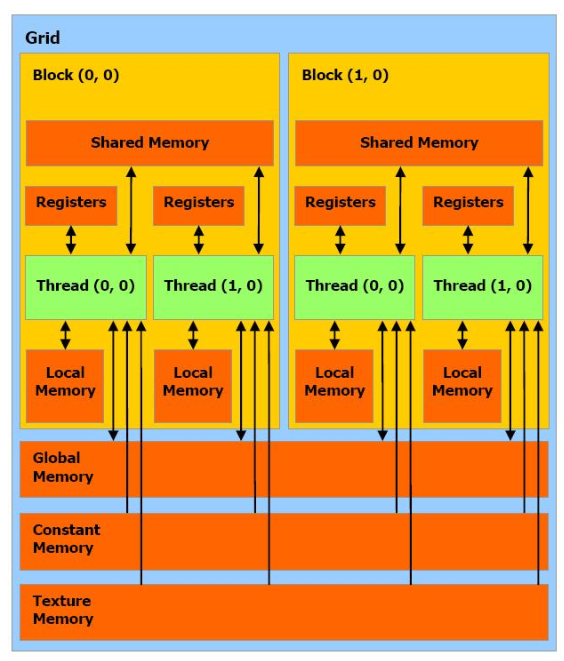
\includegraphics[width=0.6\textwidth,height=\textheight]{source/figures/sw_model_memory.png}
\caption{Memory hierarchy {[}11{]}. \label{img:sw_model_memory}}
\end{figure}

In summary, CUDA applications solve problems that were modeled based on
\emph{divide and conquer} principle. 
Each thread executes a kernel on a small subset of data.
Thus, CUDA software model not
only allows users to achieve high computational performance, but also
high scalable CUDA applications.

\hypertarget{nvidia-gpu-hardware-model}{%
\section{NVIDIA GPU Hardware Model}\label{nvidia-gpu-hardware-model}}

The CUDA architecture is based on \textbf{Streaming Multiprocessors}
(SM) which perform the actual computation. Each SM has its own control
units, registers, execution pipelines and local memories, but they also
have access to global memory as ilustrated in Figure
\ref{img:sm_memory}. A \textbf{stream} is a queue of CUDA operations,
memory copies and kernel launches. Streams are presented in more detail in 
following sections.

\begin{figure}
\centering
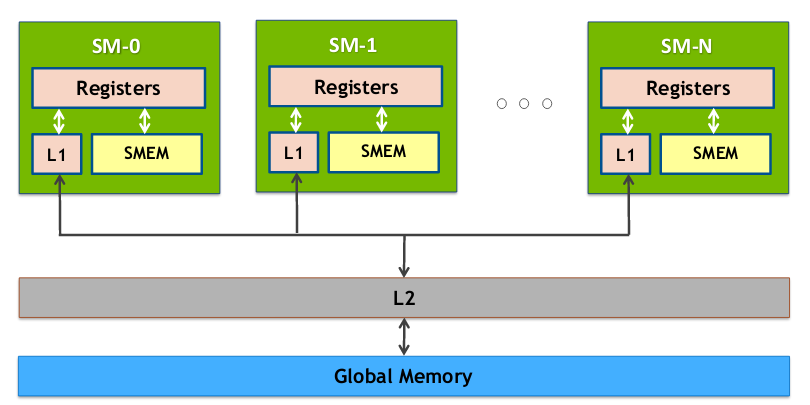
\includegraphics[width=0.6\textwidth,height=\textheight]{source/figures/sm_memory.png}
\caption{Memory hierarchy \label{img:sm_memory}}
\end{figure}

When a kernel grid is launched, blocks are enumerated and assigned to the
SMs. Once the blocks are assigned, threads are managed in \textbf{wraps}
by the \textbf{wrap scheduler}. A wrap is a group of 32 threads that
run in parallel. Thus, it is highly recommendable to use block sizes of
size \(32N, N \in \mathbb{N}\), otherwise there would be \textit{inactive}
threads. An example is shown in Figure \ref{img:inactive_thread} where
there is a block of 140 threads but since the wrap scheduler works with
wraps, 20 threads are wasted because no other block can make use of them.

\begin{figure}
\centering
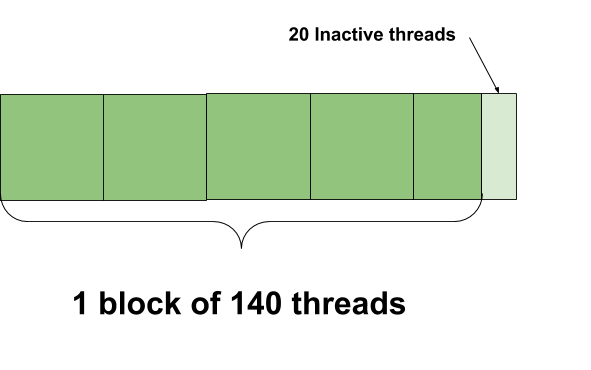
\includegraphics[width=0.6\textwidth,height=\textheight]{source/figures/inactive_thread.png}
\caption{Inactive threads \label{img:inactive_thread}}
\end{figure}

The amount of threads and blocks that can run concurrently per SM
depends on the number of 32-bit registers and shared memory within SM
as well as the CUDA computing capability of the GPU. Information related
to the maximum amount of blocks or threads as well as the computing
capability of the GPU can be displayed executing a device query
tool, which is installed by default on the Jetson TX2. 
Some information about Jetson TX2 is presented below:

\begin{Shaded}
\begin{Highlighting}[]
\ExtensionTok{CUDA}\NormalTok{ Device Query (Runtime API) }\ExtensionTok{version}\NormalTok{ (CUDART static linking)}
\ExtensionTok{Detected}\NormalTok{ 1 CUDA Capable device(s)}
\ExtensionTok{Device}\NormalTok{ 0: }\StringTok{"NVIDIA Tegra X2"}
  \ExtensionTok{CUDA}\NormalTok{ Driver Version / Runtime Version     9.0 / 9.0}
  \ExtensionTok{Total}\NormalTok{ amount of global memory:            7850 MBytes }
  \KeywordTok{(} \ExtensionTok{2}\KeywordTok{)} \ExtensionTok{SM}\NormalTok{, (128) }\ExtensionTok{CUDA}\NormalTok{ Cores/SM:             256 CUDA Cores}
  \ExtensionTok{L2}\NormalTok{ Cache Size:                            524288 bytes}
  \ExtensionTok{Total}\NormalTok{ amount of shared memory per block:  49152 bytes}
  \ExtensionTok{Total}\NormalTok{ number of registers per block:      32768}
  \ExtensionTok{Max.}\NormalTok{ number of threads per SM:            2048}
  \ExtensionTok{Max.}\NormalTok{ number of threads per block:         1024}
  \ExtensionTok{Max}\NormalTok{ dim. size of a thread block (x,y,z)}\BuiltInTok{:}\NormalTok{  (1024, 1024, 64)}
  \ExtensionTok{Max}\NormalTok{ dim. size of a grid size    (x,y,z)}\BuiltInTok{:}\NormalTok{  (2\^{}31{-}1, 65535, 65535)}
\end{Highlighting}
\end{Shaded}

\hypertarget{nvidia-jetson-tx2s-gpu-scheduler}{%
\section{NVIDIA Jetson TX2's GPU
Scheduler}\label{nvidia-jetson-tx2s-gpu-scheduler}}

It is common to use several kernels in an application. In order to reduce
computation time and maximaze GPU utilization, it is desired to run
multiple kernels in parallel. CUDA uses streams to achieve this goal. As
mentioned before, a stream is a queue of CUDA operations, memory copies
and kernel launches. Thus, it is possible either to launch multiple
kernels within one streams or multiple kernels on multiple streams.
Operations within the same stream are managed in FIFO (First In First
Out) fashion, thus,  the term \textbf{stream queue} in this work is used to refer FIFO queues within a stream. 
The Jeston TX2's GPU assigns resources to streams using its internal scheduler.

Predictability is an important characteristic of safety-critical
systems. It requires both functional and timing correctness. However, a
detailed information about the Jetson TX2's GPU scheduler behaviour is
not publicly available. Without such details, it is imposible to analyze
timing constrains. Nevertheless, there are some efforts {[}12{]},
{[}13{]} and {[}14{]} aimed at revealing these details through black-box
experimentation.

NVIDIA GPU scheduling policies depend on whether the GPU workloads are
launched by a CPU executing OS threads or OS processes. This work focuses on
the first case, because GPU computations launched by OS processes have
more unpredictable behaviours, as stated in {[}12{]} and {[}13{]}. In
this section, GPU scheduling policies devired by
{[}12{]} are presented and an example clarifies their use.

Some terms should be defined first. When one block of a kernel has been
scheduled for execution on a SM it is said that the block was
\textbf{assigned}. Moreover, it's said a kernel was \textbf{dispatched}
as soon as one of its blocks were assigned, and \textbf{fully
dispatched} once all its blocks were assigned. The same applies to copy
operations and CE.\\
There are, in addition, FIFO CE queues used to schedule copy operations
and FIFO EE queues used to schedule kernel launches. Stream queues feed
CE and EE queues. Bellow  the rules that determine scheduler and queues' behaviours are presented.

\begin{itemize}
\tightlist
\item
  \textbf{General Scheduling Rules}:

  \begin{itemize}
  \tightlist
  \item
    \textbf{G1} A copy operation or kernel is enqueued on the stream
    queue for its stream when the associated CUDA API function (memory
    transfer or kernel launch) is invoked.
  \item
    \textbf{G2} A kernel is enqueued on the EE queue when it reaches the
    head of its stream queue.
  \item
    \textbf{G3} A kernel at the head of the EE queue is dequeued from
    that queue once it becomes fully dispatched.
  \item
    \textbf{G4} A kernel is dequeued from its stream queue once all of
    its blocks complete execution.
  \end{itemize}
\item
  \textbf{Non-preemptive execution}:

  \begin{itemize}
  \tightlist
  \item
    \textbf{X1} Only blocks of the kernel at the head of the EE queue
    are eligible to be assigned.
  \end{itemize}
\item
  \textbf{Rules governing thread resources}:

  \begin{itemize}
  \tightlist
  \item
    \textbf{R1} A block of the kernel at the head of the EE queue is
    eligible to be assigned only if its resource constraints are met.
  \item
    \textbf{R2} A block of the kernel at the head of the EE queue is
    eligible to be assigned only if there are sufficient thread
    resources available on some SM.
  \end{itemize}
\item
  \textbf{Rules governing shared-memory resources}:

  \begin{itemize}
  \tightlist
  \item
    \textbf{R3} A block of the kernel at the head of the EE queue is
    eligible to be assigned only if there are sufficient shared-memory
    resources available on some SM.
  \end{itemize}
\item
  \textbf{Copy operations}:

  \begin{itemize}
  \tightlist
  \item
    \textbf{C1} A copy operation is enqueued on the CE queue when it
    reaches the head of its stream queue.
  \item
    \textbf{C2} A copy operation at the head of the CE queue is eligible
    to be assigned to the CE.
  \item
    \textbf{C3} A copy operation at the head of the CE queue is dequeued
    from the CE queue once the copy is assigned to the CE on the GPU.
  \item
    \textbf{C4} A copy operation is dequeued from its stream queue once
    the CE has completed the copy.
  \end{itemize}
\item
  \textbf{Streams with priorities}:

  \begin{itemize}
  \tightlist
  \item
    \textbf{A1} A kernel can only be enqueued on the EE queue matching
    the priority of its stream.
  \item
    \textbf{A2} A block of a kernel at the head of any EE queue is
    eligible to be assigned only if all higher-priority EE queues
    (priority-high over priority-low) are empty.
  \end{itemize}
\end{itemize}

Authors in {[}12{]} mentioned that rules related to \textbf{registry
resources} are expected to have exactly the same impact as threads and
shared-memory rules.

An example of block allocation for different kernels on the Jetson's GPU  is shown in Figure \ref{img:scheduler_blocks}.
Each rectangle represents a block: the \textit{j-th} block of kernel \textit{k} is labeled K\textit{k:j}. 
End and start time of each block are represented by its right and left boundaries. 
The height of each rectangle is the number of threads used by that block.
Dashed lines correspond to time points that are interesting for analysis. 
Figure \ref{img:scheduler_queues} presents the state of queries for each time represented by dashed lines and in Tables 2.2, 2.3 and 2.4 a description of how each  scheduling rule influence queries' behaviour.

\begin{figure}
\centering
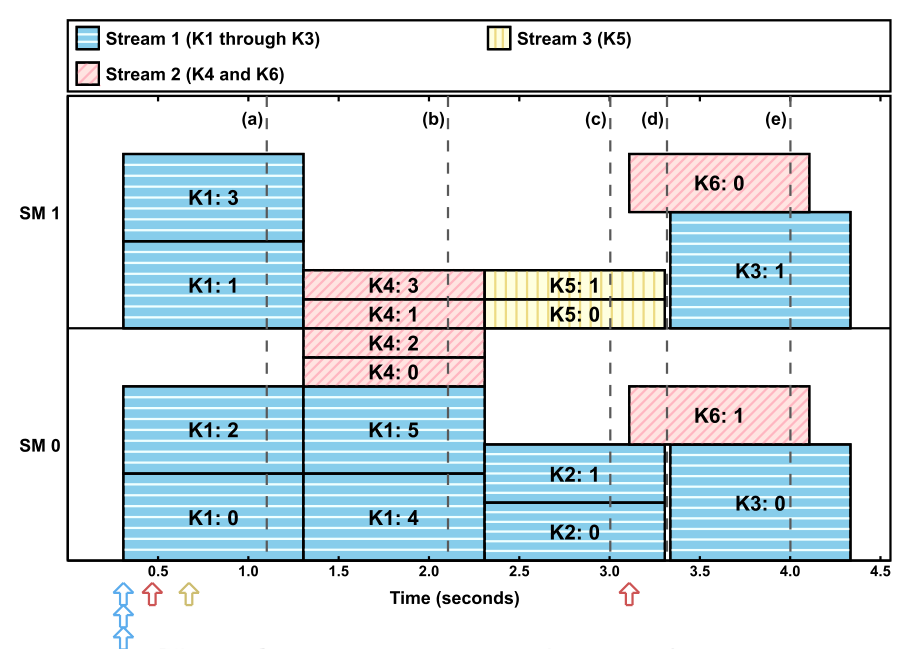
\includegraphics[width=0.6\textwidth,height=\textheight]{source/figures/scheduler_blocks.png}
\caption{Basic GPU scheduling experiment {[}12{]}
\label{img:scheduler_blocks}}
\end{figure}

\begin{figure}
\centering
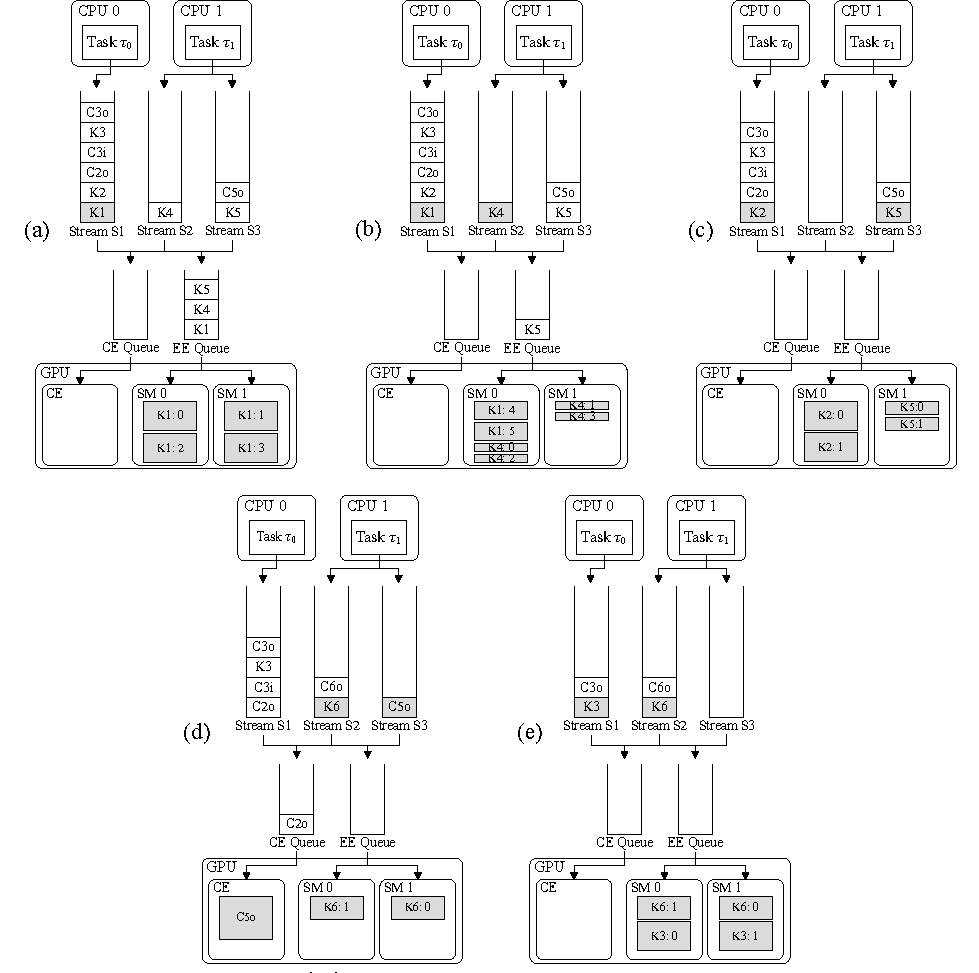
\includegraphics[width=1\textwidth,height=\textheight]{source/figures/scheduler_queues.png}
\caption{Detailed state information at various time points in Fig.
\ref{img:scheduler_blocks} {[}12{]} .\label{img:scheduler_queues}}
\end{figure}

\begin{table}[hbtp]
\small
\begin{tabularx}{\linewidth}{|X|X|X|X|X|}
    \hline
Rules & (a) t=1.0s & (b) t=2.1s & (c) t=3.0s & (d) t=3.4s \\ \hline
G1 & All Kernels except for \(\tau_6\) were enqueued on their streams. \(\tau_6\) is launched at t = 3.2s & \(\tau_6\) operations are not yet enqueued on  S2. Same reason as in (a). & Same situation as in (b). & \(\tau_6\) operations were enqueued at t=3.2s on S2. \\ \hline
G2 & \(\tau_1\), \(\tau_4\), \(\tau_5\) were at the head of their streams. They were enqueued on EE queue. & There are not new kernel at the head of stream queues. & \(\tau_2\) was enqueued on EE queue. & \(\tau_6\) kernel was enqueued on EE, because it was at the head of S2. \\ \hline
G3 & No kernels fullfill this rule. & \(\tau_1\), \(\tau_4\) have dispatched all their blocks. \(\tau_5\) is the only one on the EE queue. & \(\tau_5\), \(\tau_2\) were dequeued from EE queue, because all their blocks were dispatched.  & \(\tau_6\) was fully dispatched, thus was dequeued from EE queue. \\ \hline
G4 & No kernels fullfill this rule. \(\tau_1\) still has running blocks. & \(\tau_1\), \(\tau_4\) still have running blocks. Thus they cannot be dequeued from their stream queues. & \(\tau_1\), \(\tau_4\) were dequeued from their stream queues, because all their blocks finished execution. \(\tau_2\), \(\tau_5\) still have running blocks, they cannot be dequeued from stream queues. & \(\tau_6\) still have running blocks. Thus cannot be yet dequeued from S2. \\ \hline
\end{tabularx}
\label{tab:scheduler_rules1}
\caption{Detailed state information at various time points in Fig. 2.6}
\end{table}


\begin{table}[hbtp]
    \small
\begin{tabularx}{\linewidth}{|X|X|X|X|X|}
    \hline
Rules & (a) t=1.0s & (b) t=2.1s & (c) t=3.0s & (d) t=3.4s \\ \hline
X1 & \(\tau_4\) cannot be launched because of this rule, even when there are enough resources (512 threads) & \(\tau_4\) was the next kernel on the EE queue. It was launch because \(\tau_1\) already dispatched it's remaining blocks. & \(\tau_5\) blocks became eligible then dispatched. After that \(\tau_2\) blocks became eligible and then dispatched. & \(\tau_6\) blocks became eligible, because \(\tau_6\) was at the head of EE queue. \\ \hline
R1 & Applies only to \(\tau_1\). & \(\tau_5\) is eligible, but check R3 & \(\tau_5\) became eligible. \(\tau_2\) became eligible after \(\tau_5\). & There were enough resources for \(\tau_6\). \\ \hline
R2 & Applies only to \(\tau_1\). & \(\tau_5\) is eligible, but check R3 & There were enough thread resources for \(\tau_2\) and \(\tau_5\) (1024 threads in SM0, and 1536 threads in SM1). & There were enough thread resources in each SM for \(\tau_6\) (free 512 threads per SM , each \(\tau_6\) block needed 512 threads). \\ \hline
R3 & Applies only to \(\tau_1\). & There is not enough shared memory to launch \(\tau_5\).  Each \(\tau_5\) block requires 32KB (64KB in total), but \(\tau_4\) blocks are consuming the whole shared memory available per SM (64KB). & There were enough shared memory for \(\tau_2\) and \(\tau_5\) (64KB in each SM). & \(\tau_6\) blocks required no memory shared.  \\ \hline
\end{tabularx}
\label{tab:scheduler_rules2}
\caption{Detailed state information at various time points in Fig. 2.6}
\end{table}


\begin{table}[hbtp]
\small
\begin{tabularx}{\linewidth}{|X|X|X|X|X|}
    \hline
Rules & (a) t=1.0s & (b) t=2.1s & (c) t=3.0s & (d) t=3.4s \\ \hline
C1 & No copy operations at the head of streams. & No copy operations at the head of streams. & No copy operations at the head of streams. & C5o, C2o were enqueued on CE queue. \\ \hline
C2 & No available copy operations. & No available copy operations. & No available copy operations. & C5o was assigned to CE. \\ \hline
C3 & No available copy operations. & No available copy operations. & No available copy operations. & C5o was dequeued from CE. \\ \hline
C4 & No copy operations at the head of streams. & No copy operations at the head of streams. & No copy operations at the head of streams. & C5o is still copying. Thus it cannot be dequeued from S3. \\ \hline
\end{tabularx}
\label{tab:scheduler_rules3}
\caption{Detailed state information at various time points in Fig. 2.6}
\end{table}




\newpage

\hypertarget{jetson-tx2s-gpu-scheduler-response-time-analysis}{%
\chapter{Jetson TX2's GPU scheduler response time
analysis}\label{jetson-tx2s-gpu-scheduler-response-time-analysis}}

In this chapter, the main contribution of this work is presented, the response time analysis for Jetson TX2's GPU scheduler based on the set of scheduling rules explained in the last chapter.
A task model is defined,  works assumptions are declared, and a brief introduction to GPU response time analysis is given.\\
In addition, the last sections of this chapter present examples, description of a special case of this work,  computational complexity discussion.

\hypertarget{task-model}{%
\section{Task model}\label{task-model}}

There is a set of tasks or kernels \(\tau\) of \(n\) independent kernels
\(\{\tau_1, \tau_2, \ldots, \tau_n\}\) on a single GPU. Each kernel has
a period \(T_i\) defined as the separation between two consecutives
releases of \(\tau_i\), thread execution time workload \(C_i\) and a
grid of \(g_i\) blocks. Each block contains \(b_i\) threads.

\begin{equation} 
\tau = \{ \tau_i \}; \quad i \geq n \wedge n \in \mathbb{N}
\end{equation}

\begin{equation} 
\tau_i = \{ T_i,  C_i,  g_i,  b_i \}
\label{eq:task_def}
\end{equation}

Thus each kernel \(\tau_i\) has a total of \(g_i\cdot b_i\) threads, and
the total execution time workload of \(\tau_i\) is
\(C_i \cdot g_i \cdot b_i\). The utilization of each kernel is defined
as the total execution time workload divided by the period, as stated in
{[}15{]}.

\begin{equation} 
u_i = \frac{C_i g_i b_i}{T_i}
\label{eq:task_utilization}
\end{equation}

In addition, the total utilization of the set of tasks \(\tau\) is
defined as:

\begin{equation} 
U_t = \sum_{\tau_i \in \tau} u_i
\label{eq:task_utilization}
\end{equation}

For a kernel \(\tau_i\), \(r_i\) denotes its release  time, \(f_i\) its completion time as \(f_i\) and \(R_i = f_i - r_i\) its response time.
This work assumes that a kernel \(\tau_i\) has a deadline equal to its period \(T_i\).

\begin{figure}
\centering
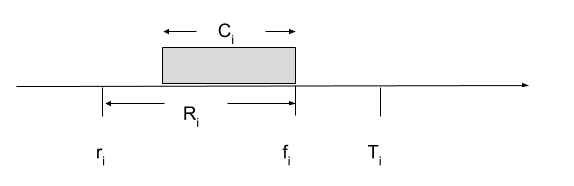
\includegraphics[width=1\textwidth,height=\textheight]{source/figures/task_timing.png}
\caption{Time chart \label{img:task_timing}}
\end{figure}

\hypertarget{assumptions}{%
\section{Assumptions}\label{assumptions}}

For the calculation of response times there are two assumption:

\hypertarget{all-blocks-have-the-same-amount-of-threads}{%
\subsection{All blocks have the same amount of
threads}\label{all-blocks-have-the-same-amount-of-threads}}

The election of the optimal number of threads for a specific kernel is a hard task.
For that reason there have been some efforts towards that
direction {[}16{]}, {[}17{]}, {[}18{]}, {[}19{]}. However, NVIDIA
developers recommend, for practical purposes, on their offical guides
{[}20{]} and {[}21{]} to use block sizes equals to either 128, 256, 512
or 1024, because it has been documented that these values are more
likely to take full advantage of the GPU resources. 
This work assumes that all the blocks, regardless the kernel, are the same size because for this work it is the first step to a more complex analysis.

\begin{equation} 
b_i = b, \quad \forall \tau_i \in \tau
\label{eq:blocksize}
\end{equation}

\hypertarget{one-big-streaming-multiprocessor}{%
\subsection{One big streaming
multiprocessor}\label{one-big-streaming-multiprocessor}}

This assumption is derived from the previous one. Each streaming
multiprocessor in the Jetson TX2 has 2048 available threads and since
\(b_i\) can be either 128, 256, 512 or 1024
(\(2048/ b_i = k, k \in \mathbb{N}\)), we can think of the two streaming
multiprocessors as a big one of 4096 threads.
It means that it could be allocated \(2048/b_i\) blocks per SM or
\(4096/b_i\) blocks in the big SM. 
Hereafter, this work asummes that Jetson TX2's GPU has only one SM.
Thus, \(g_{max}\) defines the maximum number of blocks that can be allocated in the SM at some point in time.

\begin{equation} 
g_{max} = \frac{b_{max}}{b}, \quad  g_{max} \in \mathbb{N}
\label{eq:max_grid}
\end{equation}

Where \(b_{max}\) is the maximum amount of threads in the GPU in the
case of Jetson TX2 is 4096.

\hypertarget{introduction-to-gpu-response-time-analysis}{%
\section{Introduction to GPU Response Time
Analysis}\label{introduction-to-gpu-response-time-analysis}}

In addition to the variables defined in the assumptions section, 
\(g_{f}(t)\) defines the number of blocks that are available at some point in
time \(t\), and \(t_a\) the point in time in which a block \(b_i \in g_i\) can be allocated.
In the case \(g_{f}(t)\) the time point is obvious or irrelevant \(g_{f}\) is used instead.

For example in Figure \ref{img:free_blocks}a is shown that for
\(t=t_1\) the amount of free blocks \(g_{f}\) is lower than \(g_{max}\)
while in Figure \ref{img:free_blocks}b for  \(t=t_2\),
\(g_{f} = g_{max}\).

\begin{figure}
\centering
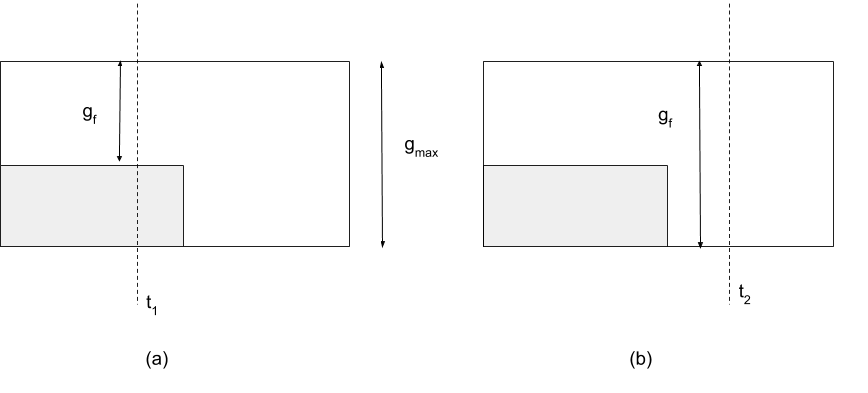
\includegraphics{source/figures/free_blocks.png}
\caption{Free blocks (a) at \(t=t_1\), \(g_f < g_{max}\) (b) at
\(t=t_2\), \(g_f = g_{max}\) \label{img:free_blocks}}
\end{figure}

In Figure \ref{img:ta_example} there are two cases for a kernel \(\tau_4\). 
The GPU scheduler allocates a block \(b_4 \in g_4\). In
Figure \ref{img:ta_example}a the release time \(r_4\) of the kernel 4 is
lower than \(t_1\), which means that \(t_a = t_1\) because
\(r_4 \leq t_1\) and kernel 3 (\(\tau_3\)) was already dequeued. In Figure
\ref{img:ta_example}b \(r_4\) lies between \(t_2\) and \(t_3\), in that
case \(t_a = r_4\), because all previous kernels were already dequeued
and there are enough resources.

\begin{figure}
\centering
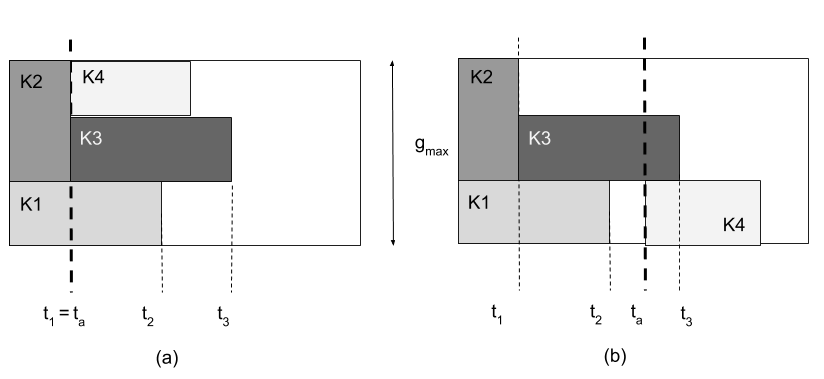
\includegraphics{source/figures/ta_example.png}
\caption{(a) \(t_a=t_1 \quad \forall r_4\) s.t \(r_4 \leq t_1\) (b)
\(t_a=r_4 \quad \forall r_4\) s.t \(t_2 \leq r_4 \leq t_3\)
\label{img:ta_example}}
\end{figure}

Assuming \(t_a\) is known, to calculate how many blocks
can be allocated at that point in time the value of \(g_f\) at \(t_a\) should be known.
In Figure \ref{img:new_kernel_1}a a new
kernel \(\tau_3\) with 6 blocks \(g_3 = 6\) is going to be allocated on the
Jetson's GPU. Each block have 512 threads, which means that
\(g_{max} = 8\). The GPU is not executing any kernel at \(t=t_a\) as
shown in Figure \ref{img:new_kernel_1}b therefore \(g_f = g_{max} = 8\)
at \(t=t_a\). Given that \(g_3 < g_f(t_a)\) all the blocks of \(\tau_3\) are
allocated at the same time as shown in Figure \ref{img:new_kernel_1}c. 
The completion time \(f_3\) of kernel \(\tau_3\) is \(t_a\) plus the thread
execution time given by \(C_3\), \(f_3 = C_3 + t_a\). If we assume that
the release time \(r_3\) is the same as \(t_a\) then the completion time
for \(\tau_3\) is the same as the response time \(R_3\), otherwise
\(R_3 \geq f_3\).

\begin{figure}
\centering
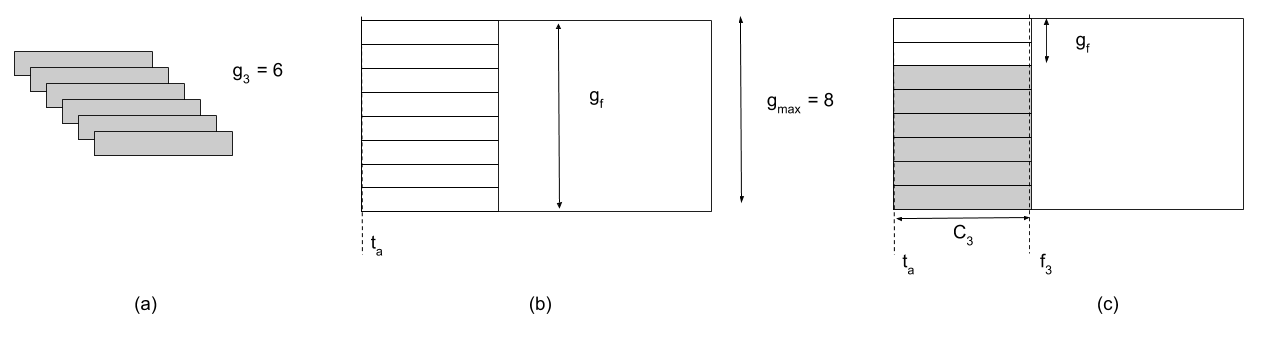
\includegraphics{source/figures/new_kernel_1.png}
\caption{(a)New kernel \(\tau_3\) with 6 blocks to allocate \(g_3 = 6\). (b)
State prior to \(\tau_3\) of the GPU (c) state after \(\tau_3\) allocation
\label{img:new_kernel_1}}
\end{figure}

Once \(f_3\) and \(R_3\) are calculated, it is important to update the
values of \(t_a\) and \(g_f\), because these values are used by the
following kernel. Let us start with \(g_f\), it is easy to notice that
after \(\tau_3\) allocation there are two free blocks \(g_f - g_3 = 2\) as a
result the new value of \(g_f = 2\). On the other hand, by definition
\(t_a\) is the point in time in which a block \(b_i \in g_i\) can be
allocated, therefore \(t_a\) will not change because \(g_f > 0\).

In Figure \ref{img:new_kernel_2} is presented another highly probable
scenario. We use the same kernel \(\tau_3\) as in the last example
(\(g_3 = 6\)). However, as shown in Figure \ref{img:new_kernel_2}b,
there are two kernels already  allocated. Kernel \(\tau_1\) with 5
allocated blocks \(g_1 = 5\) and \(\tau_2\) with 3 allocated blocks \(g_2 = 3\).
Note that these kernels have different completion time \(f_2 > f_1\).
Nevertheless, the important thing is not either \(\tau_1\) or \(\tau_2\) completion time but
the value of \(t_a\) and \(g_f\). In this example, \(t_a\) is the same
as \(\tau_1\) completion time and \(g_f\) has the same value as \(g_1\),
\(g_f = 5\). Thus, 5 blocks from \(\tau_3\) will be allocated first as shown in
Figure \ref{img:new_kernel_2}c.~

\begin{figure}
\centering
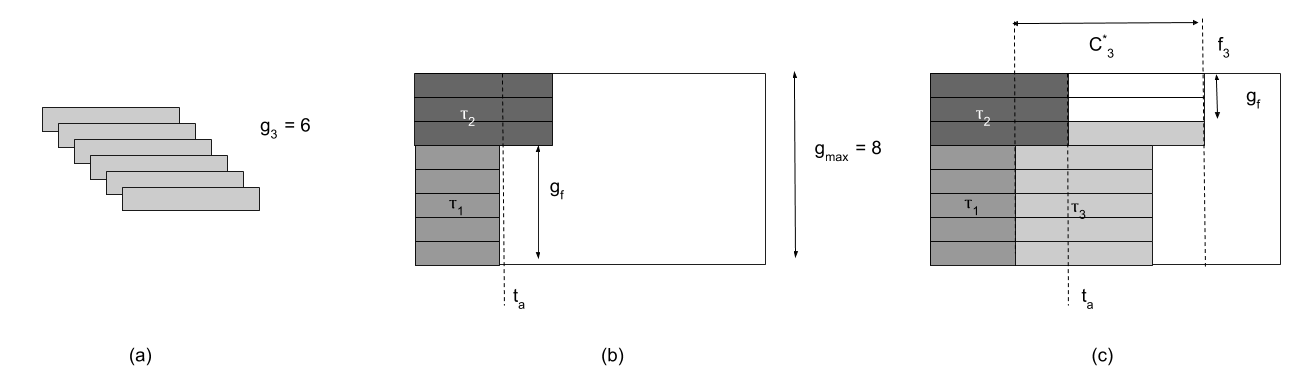
\includegraphics{source/figures/new_kernel_2.png}
\caption{(a)New kernel \(\tau_3\) with 6 blocks to allocate \(g_3 = 6\). (b)
State prior to \(tau_3\) of the GPU. Kernels \(\tau_1\) and \(\tau_2\) were previously
allocated (c) state after \(\tau_3\) allocation \label{img:new_kernel_2}}
\end{figure}

The next logical question is where the last block of \(\tau_3\) should be
allocated. The answer again is given by the updated values of \(t_a\)
and \(g_f\). 
The new value of \(t_a\) is \(f_2\) since \(f_2 <( t_a + C_3 )\), and for  \(g_f(t_a)\) is \(g_2\). 
Thus, the last \(\tau_3\) block is allocated at \(t=t_a=f_2\) and  completion time for \(\tau_3\) that is \(f_3 = f_2+C_3\) or \(f_3 = t_a + C_3\).
In Figure \ref{img:new_kernel_2}c,  \(C^{*}_3\) is the total amount of time in which \(\tau_3\) was using GPU resources.

After \(\tau_3\) is allocated, \(t_a\) and \(g_f\) should be updated again. In
this example, the new \(g_f\) is  \(g_2\) minus the last
allocated \(\tau_3\) blocks \(g_f = g_2 - 1 = 2\), while \(t_a\) remains the
same \(t_a = f_2\) because the conditions are the same as in the latter
example where there was only one kernel.

\hypertarget{response-time-analysis-algorithm}{%
\section{Response Time Analysis
Algorithm}\label{response-time-analysis-algorithm}}

This work focusses on the calculation of \(t_a\) and \(g_f\) for
each block regardless of which kernel \(\tau_i\) comes from. In addition, it is
important to note that \(t_a\) and \(g_f\) depend on how previous
blocks were allocated and on the GPU state at some point in time, as it
was described above and illustrated in the Figure \ref{img:new_kernel_1}
and Figure \ref{img:new_kernel_2}.\\
The output of our algorithm is a set of response times
\({f_1, f_2, \cdots, f_n}\) where \(n\) is the length of \(\tau\) which
values \(f_i\) depend on \(t_a\) and \(C_i\).

\begin{equation}
f_i = f(t_a, C_i)
\end{equation}

The core algorithm is described in Algorithm \ref{alg:basic}. 
This version is derived directly from the examples
illustrated in Figure \ref{img:new_kernel_1} and Figure
\ref{img:new_kernel_2}.
In other words, even for complex situations such as different release times or block sizes, this algorithm remains the same.
Thus, some details were omitted such as how \(t_a\) and \(g_f\) are updated in the case that \(g_f \geq g_i\), however the big picture of what is necessary at each step is shown.

\begin{figure}[ht]
\centering
\begin{minipage}{.7\linewidth}
    \begin{algorithm}[H]
        \DontPrintSemicolon
        \SetAlgoLined
        \SetKwInOut{Input}{Input}\SetKwInOut{Output}{Output}
        \Input{$\tau$}
        \Output{${f_1,\cdots, f_n}$}
        \BlankLine
        Initialization: $t_a = 0$, $g_f = g_{max}$, $i=1$ \\
        \While{ $i \leq n$}{
            \eIf{ $g_f \geq g_i$}{
                $f_i = t_a + C_i$; \\
                Update $g_f$ and $t_a$; \\
                i++ ; // Next kernel \\ 
            }{
                $g_i = g_i - g_f$;\\
                Update $g_f$ and $t_a$; \\
            }
        }
        \caption{Core response time analysis algorithm }
        \label{alg:basic}
    \end{algorithm} 
  \end{minipage}
\end{figure}

In order to analyze a new kernel \(\tau_i\) and update \(t_a\) and
\(g_f\) it is important to track the values of \(g_f\quad \forall t \leq t_a\).
Fortunately, it is only necessary to track \(g_f\) at specific points in
time. Some relevant points in time, as it was shown in the previous
example described by Figure \ref{img:new_kernel_2}, are given by
completion times of previous kernels. In other words 
\(g_{i-k}\) and \(f_{i-k}\) where \(k \in {1,2,\dots, i-1}\) are tracked, because
updated values of \(g_f\) and \(t_a\) depend on these as well.

A set \(h\) is defined as a values  pair \((t_k, g_k)\) where \(g_k\)
is the number of free blocks at \(t=t_k\) such that \(t_k \geq t_a\).
A further example shows step by step how this array \(h\) is
filled and updated in order to have a better understanding.

A complete version of our algorithm is presented in Algorithm
\ref{alg:full}.

\begin{figure}[ht]
\centering
\begin{minipage}{.7\linewidth}
    \begin{algorithm}[H]
        \DontPrintSemicolon
        \SetAlgoLined
        \SetKwInOut{Input}{Input}\SetKwInOut{Output}{Output}
        \Input{$\tau$}
        \Output{${f_1,\cdots, f_n}$}
        \BlankLine
        Initialization: $t_a = 0$, $g_f = g_{max}$, $i=1$, $h = \{\}$ \\
        \While{ $i \leq n$}{
            \eIf{ $g_f \geq g_i$}{
                $f_i = t_a + C_i$; \\
                $h = \{h; (f_i, g_i )\}$;\\
                $t_a = t_a$;\\ 
                $g_f = g_f - g_i$; \\
                i++ ; // Next kernel \\ 
            }{
                $g_i = g_i - g_f$;\\
                $h = \{ h; (t_a+C_i, g_f) \}$;\\
                $[ t_a, \mathrm{index}] = \mathrm{min}( h[:,1] )$;\\
                $g_f = h[ \mathrm{index}, 2]$;\\
                Update $h$;\\
            }
        }
        \caption{Response time analysis algorithm }
        \label{alg:full}
    \end{algorithm} 
  \end{minipage}
\end{figure}

Our algorithm is based on three main updates: \(h\), \(t_a\) and
\(g_f\). The set \(h\) can be seen as an array of size Nx2, where \(N\)
is the number of tracked pairs. For this reason, when \(g_f > g_i\) MATLAB notation of \texttt{min} function
\texttt{{[}value,\ index{]}\ =\ min(A)} is used, where \texttt{index} is the
position of the pair or row \((t_k, g_k) \in h\) that has the minimun of
all time values saved in \(h\). Once the pair with the minimun
time is found, \(t_a = t_k\) and \(g_f = g_k\) are assigned. It is important to
mention again that by definition of \(h\), all the tracked times should
be greater or equal than the current \(t_a\), meaning that pairs that
have tracked times lower than \(t_a\) must be removed.

\hypertarget{example}{%
\section{Example}\label{example}}

In this example there are four kernels, all with the same
period \(T = 15\) and block size of 512 threads, \(b = 512\), which
means \(g_{max} = 8\). The task is defined as
\(\tau = \{\tau_1 = \{15, 4, 2, 512\} , \tau_2 = \{15, 6,7,512\}, \tau_3 = \{15, 6,2,512\}, \tau_4 =\{ 15, 5,5,512\} \}\).

At the beginning \(t_a =0\), \(i=1\), \(h=\{\}\) and
\(g_f = g_{max} = 8\). The first one is \(\tau_1\). Kernel \(\tau_1\)
and initial state of GPU are shown in Figure \ref{img:ex_1}(a) and Figure
\ref{img:ex_1}(b) respectively.

\begin{itemize}
\tightlist
\item
  \(g_f \geq g_1\)? yes, because \(g_1 = 2\)
\item
  \(f_1 = t_a + C_1 = 0 + 4 = 4\)
\item
  \(h = \{h, (f_1, g_1)\} = \{ (4,2) \}\)
\item
  \(t_a = 0\)
\item
  \(g_f = g_f - g_1 = 8 - 2 = 6\)
\item
  \(i = 2\)
\end{itemize}

After \(\tau_1\) allocation the GPU state is as shown in Figure
\ref{img:ex_1}(c), as it is observed, \(t_a\) remains the same but
\(g_f\) now is 6. Furthermore, that is the initial GPU state when
\(\tau_2\) arrives.

\begin{figure}
\centering
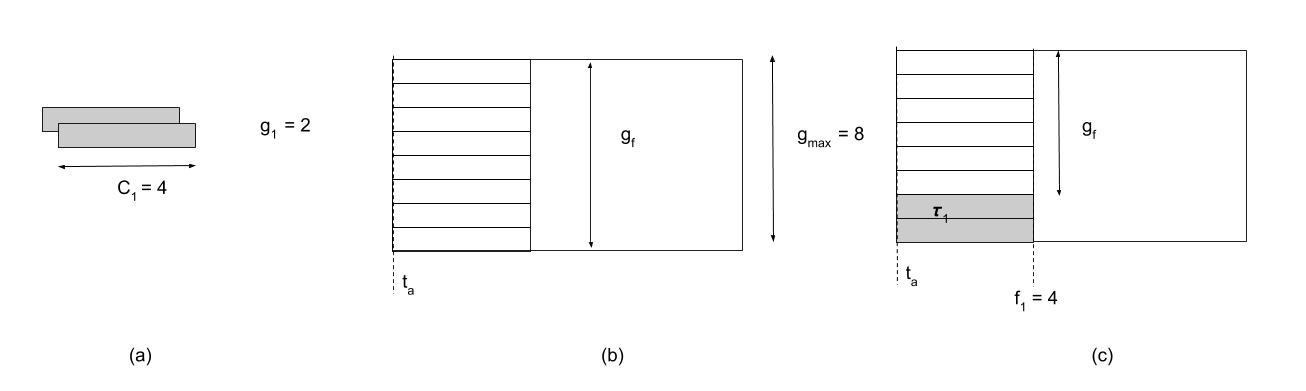
\includegraphics{source/figures/ex_1.jpg}
\caption{(a) Kernel \(\tau_1\) (b)GPU state prior to \(\tau_1\)
allocation (c) GPU state after \(\tau_1\) allocation \label{img:ex_1}}
\end{figure}

Since \(i=2\), it's time to analyze \(\tau_2\). Figure \ref{img:ex_2}(a)
shows the number of blocks that should be allocated for \(\tau_2\). It
this case \(t_a = 0\) and \(g_f = 6\) as shown in Figure
\ref{img:ex_2}(b).

\begin{itemize}
\tightlist
\item
  \(g_f \geq g_2\)? no, because \(g_i = 7\)
\item
  \(g_2 = g_2 - g_f = 7-6 = 1\)
\item
  \(h = \{h, (t_a + C_2, g_f)\} = \{ (4,2), (6,6) \}\)
\item
  \([ t_a, \mathrm{index} ] = \mathrm{min}(h[:,1]) = \mathrm{min}([4,6])\)
\item
  \([ t_a, \mathrm{index} ] = [4,1]\)
\item
  \(g_f = h[ \mathrm{index},2] = h[1,2] = 2\)
\item
  \(h = h - \{ (4,2) \} = \{ (4,2), (6,6) \} - \{ (4,2) \}\)
\item
  \(h = \{(6,6)\}\)
\end{itemize}

\begin{figure}
\centering
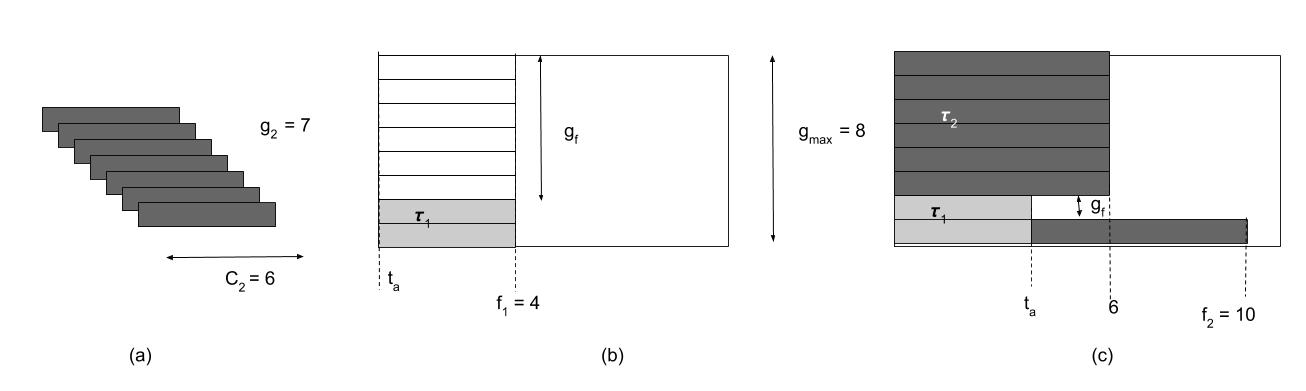
\includegraphics{source/figures/ex_2.jpg}
\caption{(a) Kernel \(\tau_2\) (b)GPU state prior to \(\tau_2\)
allocation (c) GPU state after \(\tau_2\) allocation \label{img:ex_2}}
\end{figure}

Note that the current value of \(t_a\) is the completion time of \(\tau_1\) and
\(g_f\) is \(g_1\), that is why it is important to
track \(f_1\) and \(g_1\). However, completion time for \(\tau_2\) is
not known yet. Consequently, \(\tau_2\) is still under analysis.

\begin{itemize}
\tightlist
\item
  \(g_f \geq g_2\)? yes, because \(g_2 = 1\)
\item
  \(f_2 = t_a + C_2 = 4 + 6 = 10\)
\item
  \(h = \{h, (f_2, g_2)\} = \{ (6,6),(10,1) \}\)
\item
  \(t_a = 4\)
\item
  \(g_f = g_f - g_2 = 2 - 1 = 1\)
\item
  \(i = 3\)
\end{itemize}

In Figure \ref{img:ex_2}(c) the GPU state is shown, \(t_a\) and \(g_f\)
values after \(\tau_2\) allocation. This setup is the starting point for
the analysis of \(\tau_3\) as observed in Figure \ref{img:ex_3}(b).
Since it was described a step by step analysis for \(\tau_1\) and
\(\tau_2\), some details in \(\tau_3\) analysis are skipped, however the focus is on \(h\).

\begin{figure}
\centering
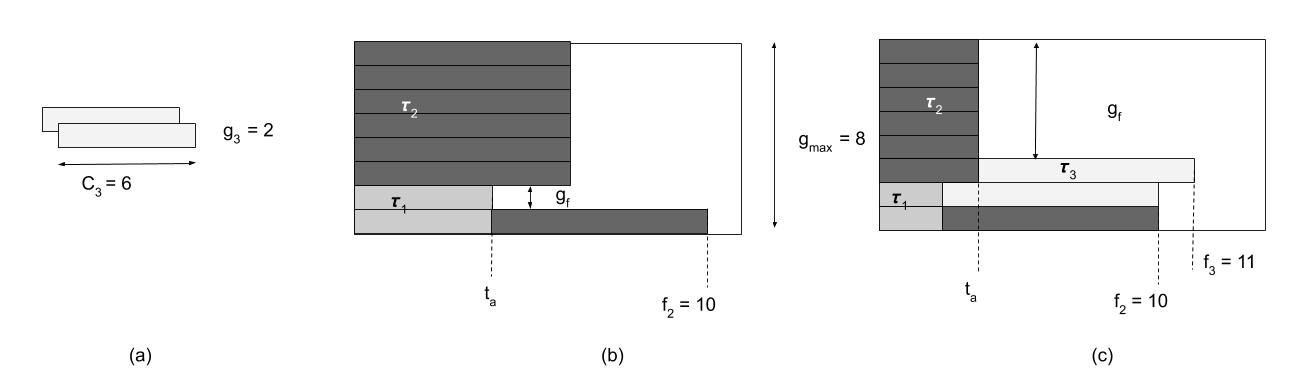
\includegraphics{source/figures/ex_3.jpg}
\caption{(a) Kernel \(\tau_3\) (b)GPU state prior to \(\tau_3\)
allocation (c) GPU state after \(\tau_3\) allocation \label{img:ex_3}}
\end{figure}

The initial setup for \(\tau_3\) is \(t_a = 4\), \(g_f= 1\) and
\(h = \{ (6,6),(10,1) \}\). The number of blocks and thread execution
time of \(\tau_3\) is illustrated in Figure \ref{img:ex_3}.

\begin{itemize}
\tightlist
\item
  \(g_f \geq g_3\)? no
\item
  \(g_3 = g_2 - g_f = 1\)
\item
  \(h = \{ (6,6), (10,1), (10,1) \}\)
\item
  \(h = \{ (6,6), (10,2) \}\)
\item
  \([ t_a, \mathrm{index} ] = [6,1]\)
\item
  \(g_f = h[ \mathrm{index},2] = h[1,2] = 6\)
\item
  \(h = \{(10,2)\}\)
\end{itemize}

Note the \emph{extra} step with \(h\) in which
\(h\) went from having three pairs to having just two. The reason behind
it lies on the definition of \(h\). The set \(h\) of pair of values
\((t_k, g_k)\) where \(g_k\) are the number of free blocks at \(t=t_k\);
note that at \(t=10\) there are two allocated blocks, one
that comes from \(\tau_2\) and one from \(\tau_3\) as shown is Figure
\ref{img:ex_3}(c) as well as the results of the following \(\tau_3\)
analysis.

\begin{itemize}
\tightlist
\item
  \(g_f \geq g_3\)? yes
\item
  \(f_3 = t_a + C_3 = 12\)
\item
  \(h = \{ (10,2),(12,1) \}\)
\item
  \(t_a = 6\)
\item
  \(g_f = g_f - g_3 = 5\)
\item
  \(i = 4\)
\end{itemize}

The analysis for \(\tau_4\) is trivial. The blocks for \(\tau_4\), GPU state prior to \(\tau_4\) allocation and GPU state after \(\tau_4\) allocation are shown in Figure \ref{img:ex_4}. 
The completion time \(f_4\) is 11.

\begin{figure}
\centering
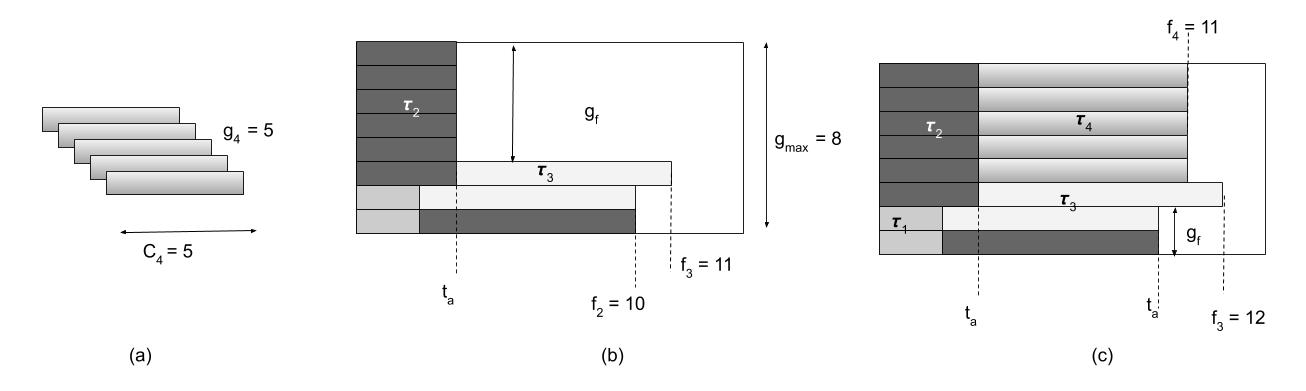
\includegraphics{source/figures/ex_4.jpg}
\caption{(a) Kernel \(\tau_4\) (b)GPU state prior to \(\tau_4\)
allocation (c) GPU state after \(\tau_4\) allocation \label{img:ex_4}}
\end{figure}

The completion times \(f_i \quad \forall \tau_i \in \tau\), \(f = \{4,10,12,11\}\), were explained.
Given the fact that all kernels were scheduled at the same time, the release time for
all kernels is 0. Thus, the response time for each kernel is the same as
their completion times. 
Furthermore,  all the kernels can be scheduled because \(R_i \leq T \quad \forall \tau_i \in \tau\).

\hypertarget{a-special-case}{%
\section{A Special case}\label{a-special-case}}

In this section, it is demostrated  that if all kernels are released at the
same time and also have the same thread execution time,
\(C_i = C \quad \forall i \in \tau\), then the response time analysis has not
algorithmic behavior, instead it is a set of three equations.

In this special case, there is no need of \(h\), because \(t_a\) and
\(g_f\) can be calculated directly with two equations.
In order to find \(t_a\), \(g_f\) and \(f_i\) the fact that \(C_i\) is the same for all kernels is exploitde. 
The case in which \(g_i \leq g_f\) is trivial to analyze, therefore it is skipped.
In Figure \ref{img:free_blocks_alg} the block
distribution when \(g_i > g_f\) is shown, thus in order to find \(g^{*}_f\) and
\(t^{*}_a\), that are the updated values of \(g_f\) and \(t_a\), a variable \(K\) must be calculated.

\begin{figure}
\centering
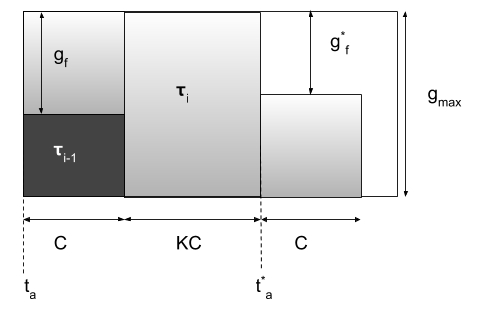
\includegraphics{source/figures/free_blocks_alg.png}
\caption{New kernel allocation \label{img:free_blocks_alg}}
\end{figure}

The value of \(K\) is given by equation \ref{eq:K}. The
interpretation is that \(K\) is the maximum amount of times that
\(g_{max}\) blocks can be allocated.

\begin{equation}
K = \lfloor \frac{g_i - g_f}{g_{max}} \rfloor
\label{eq:K}
\end{equation}

From \(K\), the value of \(g^{*}_f\) is calculated using equation \ref{eq:g_f}. 
The value of \(g^{*}_f\) can be calculated using geometry in Figure \ref{img:free_blocks_alg}.
The area of the first block is \(g_f\), of the second one \(Kg_{max}\) and the last one is \(g_i - g_f - K g_{max}\).

\begin{equation}
g^{*}_f = g_{max} - (g_i -  g_f - K g_{max} )
\label{eq:g_f}
\end{equation}

The value of \(t^{*}_a\) is calculated in a similar fashion and is given
in equation \ref{eq:t_a}. On the other hand, the calculation of \(f_i\)
remains the same.

\begin{equation}
t^{*}_a = t_a + C+ KC
\label{eq:t_a}
\end{equation}

At this point updated values of \(t_a\) and \(g_f\) are calculated with equations.
Nonetheless, there is still an algoritmic behavior given by the \texttt{if} condition. 
However the absolute value and the signum function solve this problem. 
The signum function of a real number x is defined as follows:

\begin{equation}
\mathrm{sgn}(x)=
    \begin{cases}
        -1  & \text{if    x<0,}\\
        0   & \text{if    x=0,}\\
        1   & \text{if    x>0.}
    \end{cases} 
\end{equation}

The new definition of  \(K\) is given in equation \ref{eq:new_k},
The absolute value in \ref{eq:new_k} make K to be zero when \(g_i \leq g_f\).

\begin{equation}
K = \lfloor \frac{ \| g_i - g_f \|}{g_{max}} \rfloor
\label{eq:new_k}
\end{equation}

The equation \ref{eq:alpha} defines a variable \(\alpha\).
The value of \(\alpha\) is zero when \(g_i \leq g_f\) and one otherwise.

\begin{equation}
\alpha =  \frac{ \mathrm{sgn}(g_i-g_f) + 1 }{2}
\label{eq:alpha}
\end{equation}

With \ref{eq:new_k} and \ref{eq:alpha} the \texttt{if} condition and at the same time the algoritmic behavior disappears. 
Therefore, the updated values of \(t_a\) and \(g_f\) are calculated using
\ref{eq:new_t_a} and \ref{eq:new_g_f}. 
It is important to mentiotn that  when
\(g_i \leq g_f\) \ref{eq:new_t_a} and \ref{eq:new_g_f} are the same steps described in Algorithm \ref{alg:full}.

\begin{equation}
t_a = t_a + \alpha C+ KC
\label{eq:new_t_a}
\end{equation}

\begin{equation}
g_f = \alpha g_{max} - (g_i -  g_f - K g_{max} )
\label{eq:new_g_f}
\end{equation}

\hypertarget{computational-complexity}{%
\section{Computational Complexity}\label{computational-complexity}}

The algorithm described in Algorithm \ref{alg:full} has two branches,
inside the \texttt{while} loop, given by an \texttt{if} conditional. In
Table \ref{tab:bigO} is shown the computational complexity of each step
of the real time analysis algorithm.

\begin{longtable}[]{@{}lll@{}}
\caption{Computational Complexity \label{tab:bigO}}\tabularnewline
\toprule
\begin{minipage}[b]{0.52\columnwidth}\raggedright
Step\strut
\end{minipage} & \begin{minipage}[b]{0.24\columnwidth}\raggedright
Type of operation\strut
\end{minipage} & \begin{minipage}[b]{0.15\columnwidth}\raggedright
Average Cost\strut
\end{minipage}\tabularnewline
\midrule
\endfirsthead
\toprule
\begin{minipage}[b]{0.52\columnwidth}\raggedright
Step\strut
\end{minipage} & \begin{minipage}[b]{0.24\columnwidth}\raggedright
Type of operation\strut
\end{minipage} & \begin{minipage}[b]{0.15\columnwidth}\raggedright
Average Cost\strut
\end{minipage}\tabularnewline
\midrule
\endhead
\begin{minipage}[t]{0.52\columnwidth}\raggedright
\(f_i = t_a + C_i\)\strut
\end{minipage} & \begin{minipage}[t]{0.24\columnwidth}\raggedright
Sum\strut
\end{minipage} & \begin{minipage}[t]{0.15\columnwidth}\raggedright
O(1)\strut
\end{minipage}\tabularnewline
\begin{minipage}[t]{0.52\columnwidth}\raggedright
\(h = \{h; (f_i, g_i )\}\)\strut
\end{minipage} & \begin{minipage}[t]{0.24\columnwidth}\raggedright
Append\strut
\end{minipage} & \begin{minipage}[t]{0.15\columnwidth}\raggedright
O(1)\strut
\end{minipage}\tabularnewline
\begin{minipage}[t]{0.52\columnwidth}\raggedright
\(t_a = t_a\)\strut
\end{minipage} & \begin{minipage}[t]{0.24\columnwidth}\raggedright
Sum\strut
\end{minipage} & \begin{minipage}[t]{0.15\columnwidth}\raggedright
O(1)\strut
\end{minipage}\tabularnewline
\begin{minipage}[t]{0.52\columnwidth}\raggedright
\(g_f = g_f - g_i\)\strut
\end{minipage} & \begin{minipage}[t]{0.24\columnwidth}\raggedright
Sum\strut
\end{minipage} & \begin{minipage}[t]{0.15\columnwidth}\raggedright
O(1)\strut
\end{minipage}\tabularnewline
\begin{minipage}[t]{0.52\columnwidth}\raggedright
i++\strut
\end{minipage} & \begin{minipage}[t]{0.24\columnwidth}\raggedright
Sum\strut
\end{minipage} & \begin{minipage}[t]{0.15\columnwidth}\raggedright
O(1)\strut
\end{minipage}\tabularnewline
\begin{minipage}[t]{0.52\columnwidth}\raggedright
\(g_i = g_i - g_f\)\strut
\end{minipage} & \begin{minipage}[t]{0.24\columnwidth}\raggedright
Sum\strut
\end{minipage} & \begin{minipage}[t]{0.15\columnwidth}\raggedright
O(1)\strut
\end{minipage}\tabularnewline
\begin{minipage}[t]{0.52\columnwidth}\raggedright
\(h = \{ h; (t_a+C_i, g_f) \}\)\strut
\end{minipage} & \begin{minipage}[t]{0.24\columnwidth}\raggedright
Append\strut
\end{minipage} & \begin{minipage}[t]{0.15\columnwidth}\raggedright
O(1)\strut
\end{minipage}\tabularnewline
\begin{minipage}[t]{0.52\columnwidth}\raggedright
\([ t_a, \mathrm{index}] = \mathrm{min}( h[:,1] )\)\strut
\end{minipage} & \begin{minipage}[t]{0.24\columnwidth}\raggedright
Min\strut
\end{minipage} & \begin{minipage}[t]{0.15\columnwidth}\raggedright
O(n)\strut
\end{minipage}\tabularnewline
\begin{minipage}[t]{0.52\columnwidth}\raggedright
\(g_f = h[ \mathrm{index}, 2]\)\strut
\end{minipage} & \begin{minipage}[t]{0.24\columnwidth}\raggedright
Index\strut
\end{minipage} & \begin{minipage}[t]{0.15\columnwidth}\raggedright
O(1)\strut
\end{minipage}\tabularnewline
\bottomrule
\end{longtable}

The first branch is when \(g_f \geq g_i\). The computational complexity,
given by big O notation, of that branch is O(1), because all the
operations in this branch are O(1).

In the case of the second branch the computational complexity is O(n),
because \texttt{min} function is the most costly operation. In the worst
case scenario \texttt{n} is the number of kernels we want to allocate,
it is important to highlight that only on the first branch the lenght of
\(h\) increases. Thus, the computational complexity of the \texttt{if}
statement is O(n).

The analysis of the outer \texttt{while} loop goes as follows. The number of iterations
depends on number of kernels, their grid sizes \(g_i\) and how many
blocks can be allocated in total in the GPU or \(g_{max}\). An
estimation can be given by \(\frac{g}{g_{max}}\), where \(g\) is
\(\sum g_i\), \(g\) contains the information about number of kernels and
their grid sizes. Thus, computational complexity of our algorithm is O(
\(\frac{ng}{g_{max}}\)).

\hypertarget{app4mc-implementation}{%
\section{APP4MC Implementation}\label{app4mc-implementation}}
A APP4MC implementation for AMALTHEA models is presented in this section. 
The code is presented below. 
The input is an AMALTHEA software model and the output is a \texttt{ArrayList} with completion time values for each kernel within the model. 
Runnables or kernels are assigned in line 4 to \texttt{rList}.
Temporary variables for \(c_i\), \(g_i\) and \(f\) are needed as shown in lines 6,7 and 8, and their values are assigned in lines 11 to 15. 
Since AMALTHEA software model does not have a grid size property, \texttt{CustomPropertyUtil} is used in line 14. 


Then, \(t_a\), \(g_{max}\),\(g_f\) and \(h\) should be initialized, and it is done in lines 18 to 21. 
A \texttt{HashMap} allows an easy acces to \(h\) block values, that means that time values in \(h\) are the keys.  

\lstinputlisting[style=javaCodeStyle, caption=APP4MC Implementation]{source/code/alg.java}

The algorithm itself starts at line 26. 
The first \texttt{if} statement goes from line 27 to 34.
Lists in java are a powerful tool to manage array like variable such as \(f\) and \(g_i\). 
The methods \texttt{add} and \texttt{get} make the code understandable.
The varible \(h\) is updated in line 30 using a function called \texttt{updateH} which updates the hash map with a new key and value given by \texttt{f.get(current\_kernel)} and \texttt{g\_i.get(current\_kernel)} respectively. In case the key already exists, \texttt{updateH} adds the old value andthe new value. 

The second \texttt{if} statement goes from line 35 to 46. 
In line 36 list method \texttt{set} is used to update \texttt{g\_i} value of the current kernel.
The \(h\) is updated in line 38, and the minimun key of \texttt{h} is found in line 39 using a function called \texttt{findIndexOfMinValue}. This function compares all the keys saved in \texttt{h} and returns the lowest one.
The lowest key is used to get \(g_f\) and \(t_a\) in lines 41 and 42 respectively. 
At the end the useless key is removed using HashMap method \texttt{remove(key)}.

\hypertarget{experimental-results}{%
\chapter{Experimental Results}\label{experimental-results}}

In this chapter experimental results are presented. A complete example
using AMALTHEA models can be found in the Appendix 1. There is a comparison 
between data from Jetson TX2 platfrom againts the APP4MC implementation. The former
are used as ground truth to verify our implementation and assumptions.

\hypertarget{ground-truth-generation}{%
\section{Ground truth generation}\label{ground-truth-generation}}

Amert et. al {[}12{]} published their code in github. They developed a
CUDA Scheduling Viewer, which is a tool for examining block-level
scheduling behavior and co-scheduling performance on CUDA devices. 
Inputs are configuration files on the JSON format, and the output can be
displayed as a figure using a Python script, which is provided as well. An
example output is shown in Figure \ref{img:nvidia-base}

The test scenario consists of four kernels defined as \(\tau = \{\tau_1 = \{15, 4, 2, 512\} , \tau_2 = \{15, 6,7,512\}, \tau_3 = \{15, 6,2,512\}, \tau_4 =\{ 15, 5,5,512\} \}\).
The GPU parameters were: block size = 512 threads, and \(g_{max} = 8\).

\begin{figure}
\centering
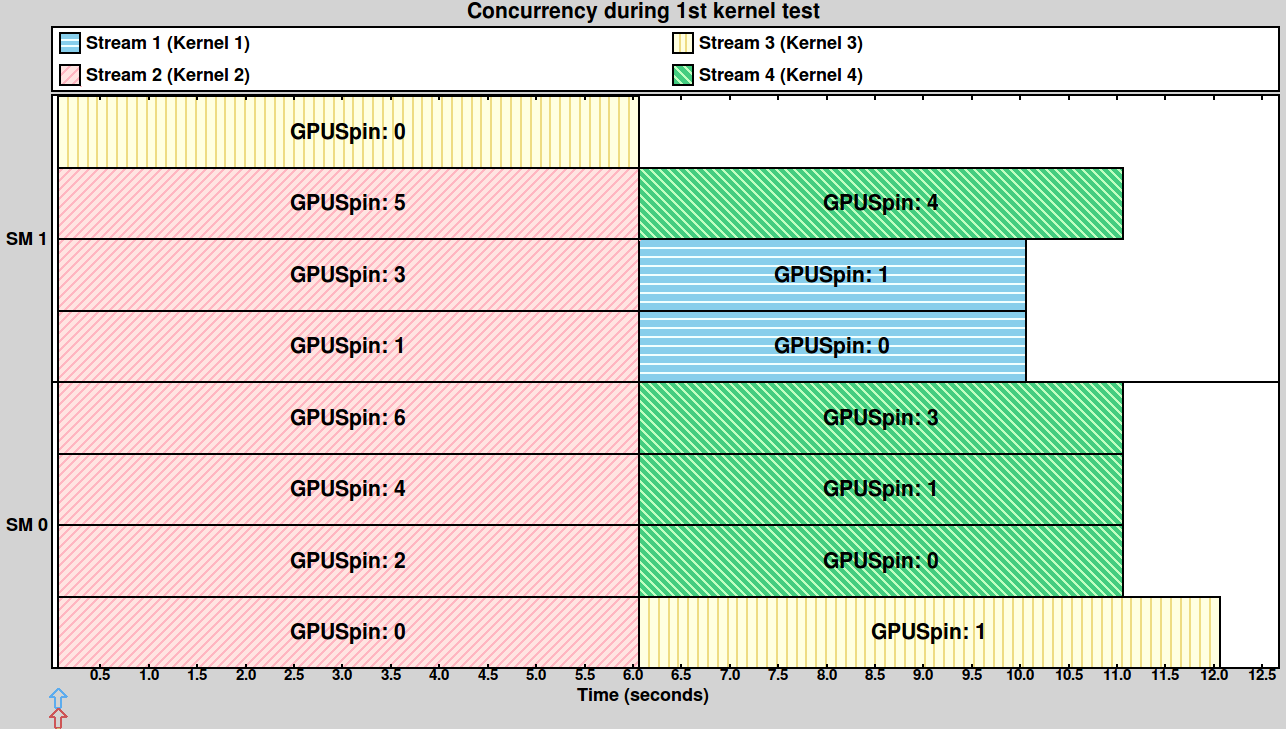
\includegraphics{source/figures/nvidia/base.png}
\caption{Output of the CUDA Scheduling Viewer \label{img:nvidia-base}}
\end{figure}

An example of a kernel description in the configuration file is as
follows:

\begin{Shaded}
\begin{Highlighting}[]
      \ErrorTok{"filename":} \ErrorTok{"./bin/timer\_spin.so",}
      \ErrorTok{"log\_name":} \ErrorTok{"k3.json",}
      \ErrorTok{"label":} \ErrorTok{"Kernel} \ErrorTok{3",}
      \ErrorTok{"thread\_count":} \ErrorTok{512,}
      \ErrorTok{"block\_count":} \ErrorTok{2,}
      \ErrorTok{"additional\_info":} \ErrorTok{6000000000}
\end{Highlighting}
\end{Shaded}

The \texttt{filename} is the benchmark kernel as binary file.
For all the kernels the binary file is \texttt{timer\_spin.so}. This file defines a
CUDA benchmark which spins waiting for a user-specified
amount of time to complete. The execution time in nanoseconds or \(C_i\)
is set as \texttt{additional\_info}. The \texttt{log\_name} is the
JSON file that contains metadata and results related to a specfied
kernel (\texttt{label}). In addition, \texttt{thread\_count} and
\texttt{block\_count} were the values of \(b_i\) and \(g_i\)
respectively.

\hypertarget{implementation-results}{%
\section{Implementation results}\label{implementation-results}}

This work is implemented in  Eclipse APP4MC as described in Section 3.8. The goal was not to test
how many kernel the Jetson could manage, instead it was focused on verifying
assumptions and therefore the algorithm.

There are  three test scenarios. The four previously described kernels
were launched in different order. The first scenario is the one
presented in Figure \ref{img:nvidia-base}. The kernels are launched on
the following order: \(\tau_2\), \(\tau_3\), \(\tau_4\), \(\tau_1\). As it is showed in Figure
\ref{img:nvidia-base} the completion times were \(f = \{6, 12,11,10\}\).
The results from APP4MC are shown in Figure \ref{img:octave-base}.

\begin{figure}
\centering
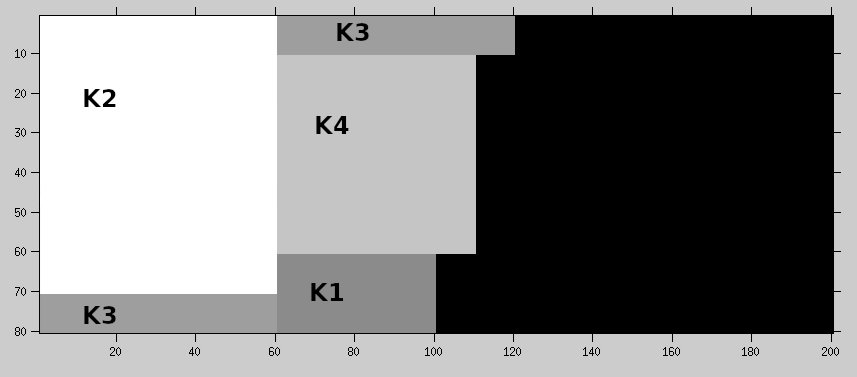
\includegraphics[width=1\textwidth,height=\textheight]{source/figures/octave/base.png}
\caption{APP4MC: Scenario 1 - \(\tau_2\),\(\tau_3\),\(\tau_4\),\(\tau_1\) \label{img:octave-base}}
\end{figure}

In the second scenario kernels were launched on the following order: \(\tau_2\),
\(\tau_4\), \(\tau_1\), \(\tau_3\). As observed in Figure \ref{img:nvidia-ex02} the completion
times were \(f = \{6,11,10,12\}\). Notice that \emph{GPUSping: 5} for
kernel 4 should be shown, but there is a bug in the code from {[}12{]}
in which sometimes the log file does not contain all the data. On the
other hand, results from APP4MC are shown in Figure
\ref{img:octave-ex02}. The block allocation visually differs from Jetson's
allocation because our code follows our assumption described in section
3.3.2. However, it can be observed that in both cases the data is exactly the same.  

\begin{figure}
\centering
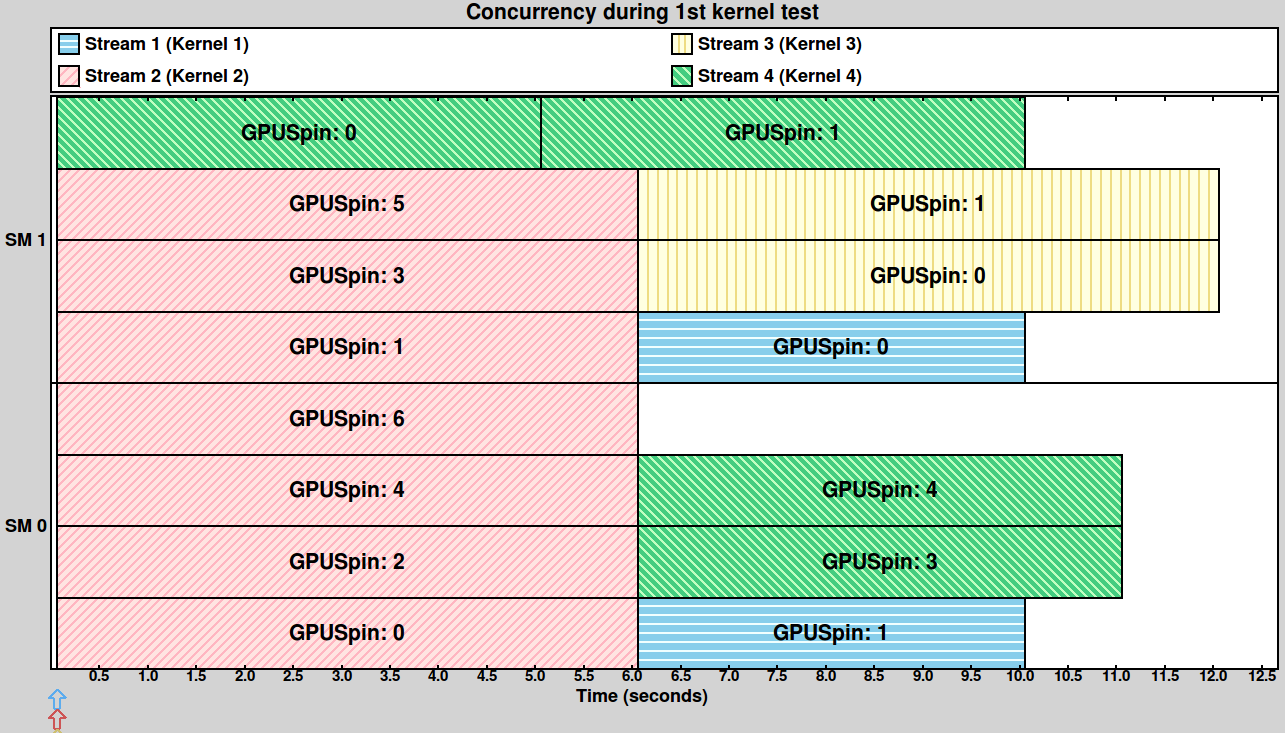
\includegraphics[width=1\textwidth,height=\textheight]{source/figures/nvidia/ex02.png}
\caption{JetsonTX2: Scenario 2 - \(\tau_2\),\(\tau_4\),\(\tau_1\),\(\tau_3\) \label{img:nvidia-ex02}}
\end{figure}

\begin{figure}
\centering
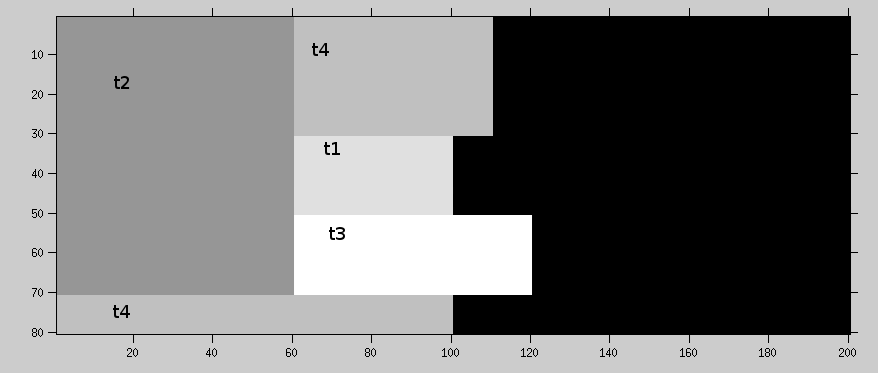
\includegraphics[width=1\textwidth,height=\textheight]{source/figures/octave/ex02.png}
\caption{APP4MC: Scenario 2 - \(\tau_2\),\(\tau_4\),\(\tau_1\),\(\tau_3\) \label{img:octave-ex02}}
\end{figure}

In the third scenario kernels are launched on the following order: \(\tau_2\),
\(\tau_1\), \(\tau_3\), \(\tau_4\). As observed in Figure \ref{img:nvidia-ex05}, completion
times are \(f = \{6,8,12,11\}\). Notice in this case that
\emph{GPUSping:4} from kernel 4 and \emph{GPUSping:1} from kernel 5
overlap in the figure. This is, again, an error on how the log file was
created. C implementation from {[}12{]} was tested using \texttt{printf}, and
the values were correct. Nevertheless, results from APP4MC shown in
Figure \ref{img:octave-ex02} remain congruent with the results of its
counterpart.

\begin{figure}
\centering
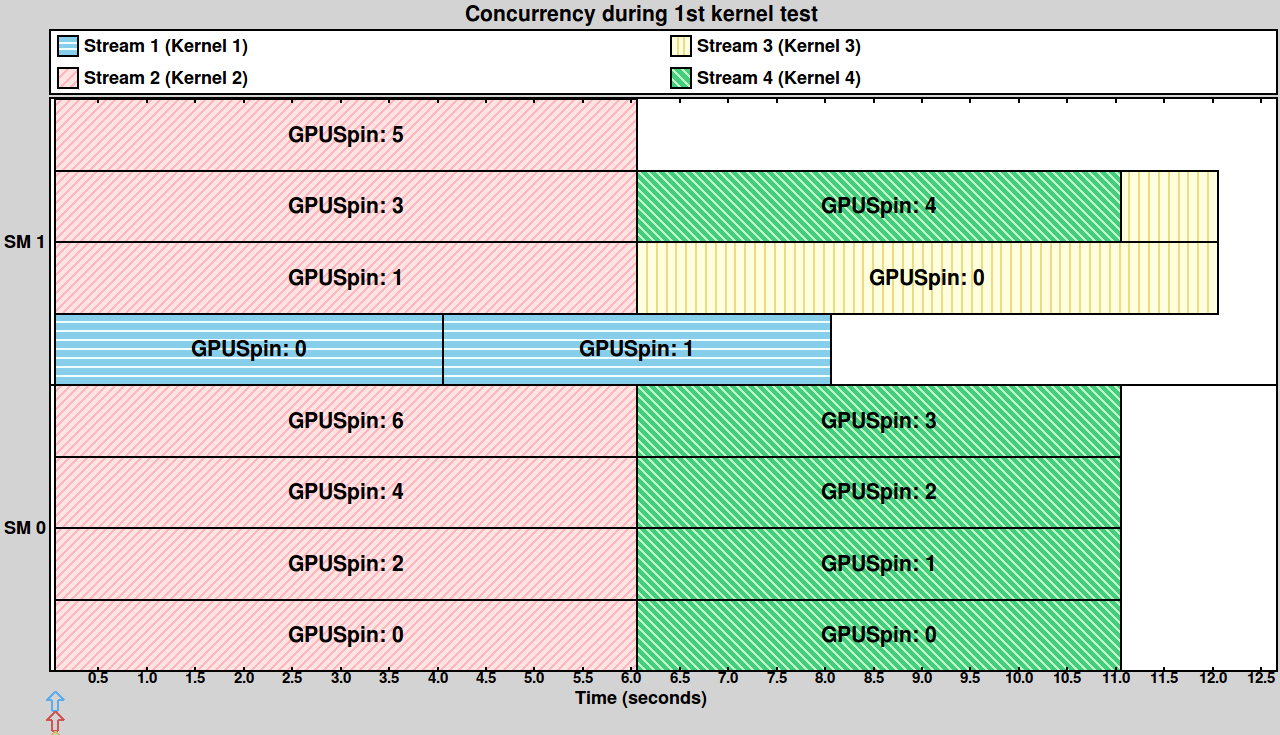
\includegraphics[width=1\textwidth,height=\textheight]{source/figures/nvidia/ex05.png}
\caption{JetsonTX2: Scenario 3 - \(\tau_2\),\(\tau_1\),\(\tau_3\),\(\tau_4\) \label{img:nvidia-ex05}}
\end{figure}

\begin{figure}
\centering
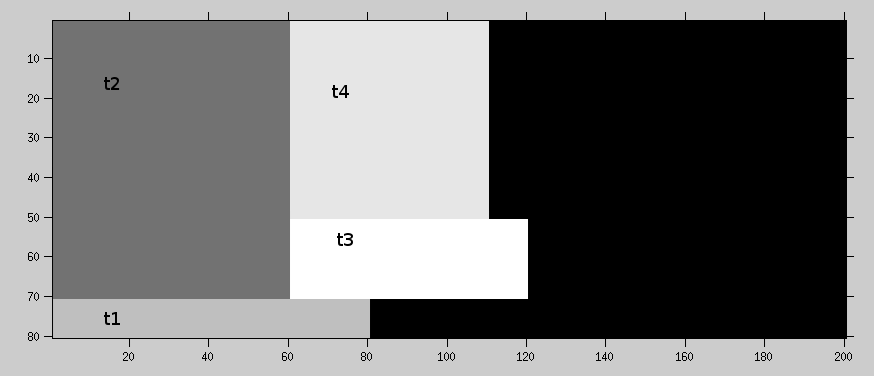
\includegraphics[width=1\textwidth,height=\textheight]{source/figures/octave/ex05.png}
\caption{APP4MC: Scenario 3 - \(\tau_2\),\(\tau_1\),\(\tau_3\),\(\tau_4\) \label{img:octave-ex05}}
\end{figure}

\hypertarget{block-analysis}{%
\section{Block analysis}\label{more-results}}

In this section the focus is on the interaction between kernels with several blocks, and kernels with long execution time.

In Figure \ref{img:nvidia-ex06} can be observed the result after
executing five kernels. The kernels are defined as follows:

\begin{itemize}
\tightlist
\item
  \(\tau_1 = \{15,4,2,512\}\): small block count, short execution time.
\item
  \(\tau_2 = \{15, 7,1,512\}\): big block count, short execution time.
\item
  \(\tau_3 = \{15,10,4,512\}\): big block count, long execution time.
\item
  \(\tau_4 =\{ 15, 1,11,512\}\): small block count, very long execution
  time.
\item
  \(\tau_5 = \{15,3,6,512\}\): big block count, medium execution time.
\end{itemize}

The result shown in Figure \ref{img:octave-ex06} is still consistent
with the ground truth. Completions times are the same for each kernel.

\begin{figure}
\centering
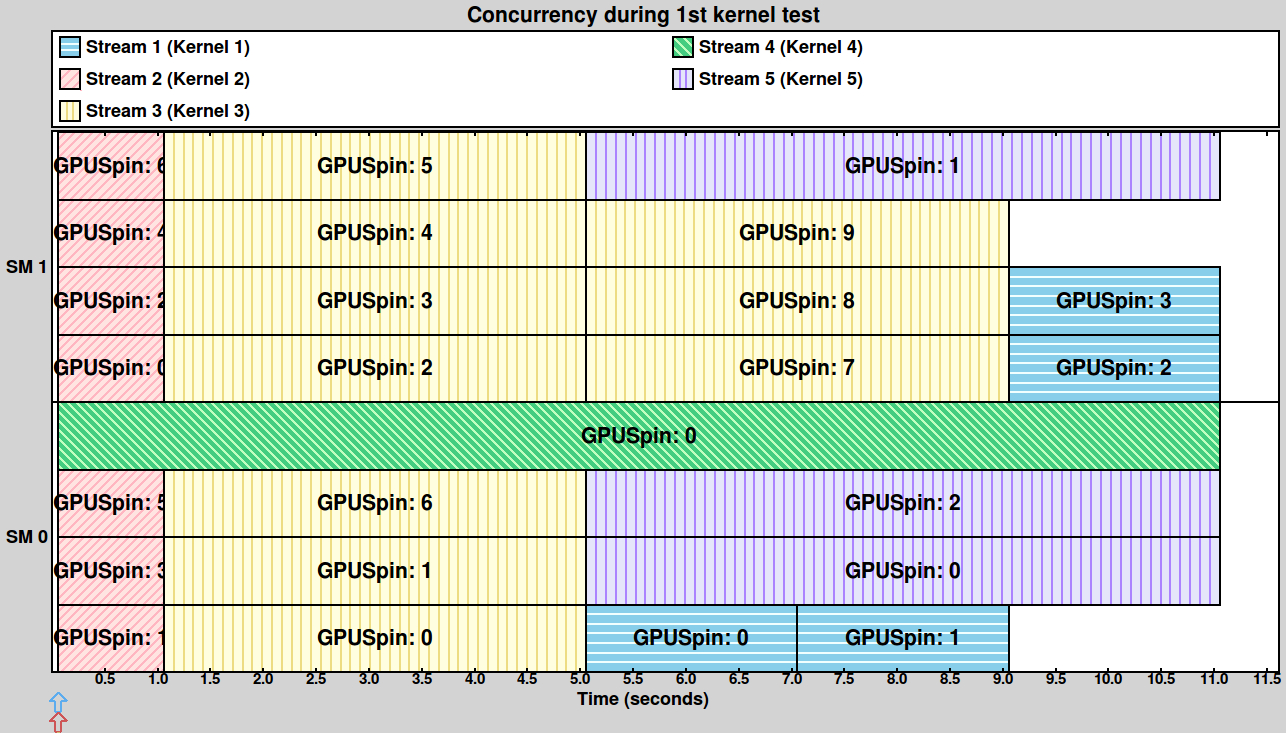
\includegraphics[width=1\textwidth,height=\textheight]{source/figures/nvidia/ex06.png}
\caption{JetsonTX2 \label{img:nvidia-ex06}}
\end{figure}

\begin{figure}
\centering
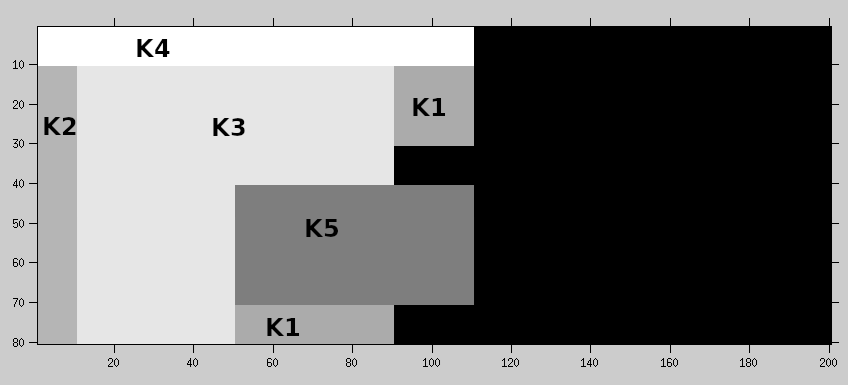
\includegraphics[width=1\textwidth,height=\textheight]{source/figures/octave/ex06.png}
\caption{APP4MC \label{img:octave-ex06}}
\end{figure}

In this experiment the setup is as follows:

\begin{itemize}
\tightlist
\item
  \(\tau_1 = \{15,5,1.5,512\}\): small block count, small execution
  time.
\item
  \(\tau_2 = \{15,4,1.5,512\}\): small block count, small execution
  time.
\item
  \(\tau_3 = \{15,7,1.5,512\}\): big block count, small execution time.
\item
  \(\tau_4 =\{ 15, 1,4,512\}\): very small block count, big execution
  time.
\item
  \(\tau_5 = \{15,8,2.5,512\}\): big block count, large execution time.
\end{itemize}

As expected completion times shown in Figure \ref{img:nvidia-ex07} and
Figure \ref{img:octave-ex07} are the same for each kernel.

\begin{figure}
\centering
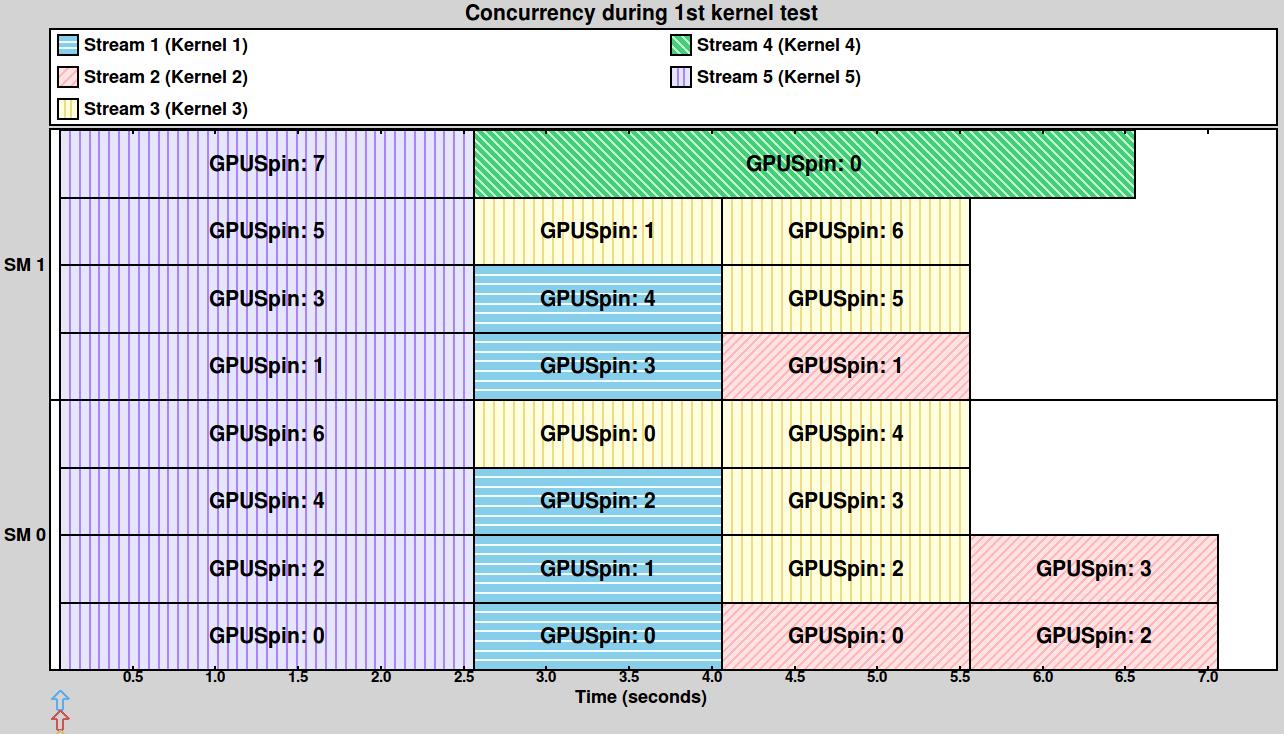
\includegraphics[width=1\textwidth,height=\textheight]{source/figures/nvidia/ex07.png}
\caption{JetsonTX2 \label{img:nvidia-ex07}}
\end{figure}

\begin{figure}
\centering
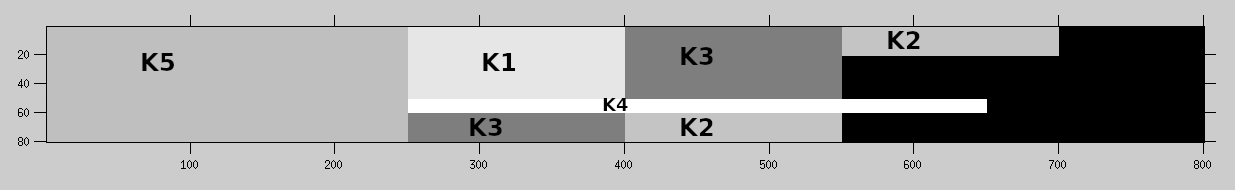
\includegraphics[width=1\textwidth,height=\textheight]{source/figures/octave/ex07.png}
\caption{APP4MC \label{img:octave-ex07}}
\end{figure}

\hypertarget{conclusion}{%
\chapter{Conclusion}\label{conclusion}}

In Chapter 1 there is an overview of the motivation of this work, the
Bosch WATERS Challenge 2019, and explained the architecture of NVIDIA Jetson
TX2 platform and its AMALTHEA model. Furthermore, in Chapter 2, 
key concepts related to NVIDIA's GPU such as kernel
definition, block and threads, as well as its memory hierarchy were introduced.
A detailed description of Jetson TX2 hardware architecture, and explantion of the
rules behind hardware scheduler were described.
In Chapter 3 the response time analysis algorithm for Jetson TX2's scheduler was presented.
In addition, some examples  explained in detail each step. 
Finally in Chapter 4 experimental results are showed.

\hypertarget{conclusions}{%
\section{Conclusions}\label{conclusions}}

For purposes of mathematical calculation, the main assumption, all blocks have the same thread count all GPU streaming multiprocessors are considered as one big streaming multiprocessor, was correct.
Experimental results show the accuracy of this work to estimate completion times for kernels executed on Jetson TX2 platform.
Moreover, an implementation in Eclipse APP4MC, which allows AMALTHEA based response time analysis for NVIDIA's Jetson TX2, was described.

\hypertarget{future-work}{%
\section{Future work}\label{future-work}}

There are several potential directions for extending this thesis. First,
the possibility to develop a complete model-based development for NVDIA
platform using AMALTHEA models, which may include automatic CUDA C code
generation for deployment and testing. Second, there is still no full
understanding of how Jetson TX2's scheduler decides which kernel should
run first. Thus, developers should either consider all possible cases
when analyzing completion times or use a reverse engineering approach to Jetson TX2's
scheduler. Finally, this work didn't consider memory transaction and other
constrains such as amount of shared memory, influence of the \emph{null}
stream and priorities within scheduler. Therefore, there is still room
for more research into this topic.

\hypertarget{appendix-1-example-app4mc}{%
\chapter*{Appendix 1: Example APP4MC}\label{appendix-1-example-app4mc}}
\addcontentsline{toc}{chapter}{Appendix 1: Example APP4MC}

Here is a complete example of how to use our response time analysis
algorithm in APP4MC to analyze AMALTHEA based Jetson TX2's models.

\lstinputlisting[style=javaCodeStyle, caption=Complete example]{source/code/rta.java}

\footnotesize

\hypertarget{references}{%
\chapter*{References}\label{references}}
\addcontentsline{toc}{chapter}{References}

\hypertarget{refs}{}
\leavevmode\hypertarget{ref-Hansen2019}{}%
{[}1{]} Paul Hansen.``BMW and Audi want to separate vehicle hardware from
software.'' 2017.[Online] Available:
\url{https://www.electronicdesign.com/automotive/bmw-and-audi-want-separate-vehicle-hardware-software}. [Accessed: 01-05-2019]

\leavevmode\hypertarget{ref-Future2019}{}%
{[}2{]} FMT. ``End to end architecture.'' 2019. [Online] Available: 
\url{https://www.future-mobility-tech.com/en/technology/end-to-end-architecture}. [Accessed: 01-05-2019]

\leavevmode\hypertarget{ref-Kanajan2006}{}%
{[}3{]} S. Kanajan, H. Zeng, C. Pinello, and A. Sangiovanni-Vincentelli,
``Exploring trade-off's between centralized versus decentralized
automotive architectures using a virtual integration environment,'' in
\emph{Proceedings of the conference on design, automation and test in
europe: Proceedings}, 2006, pp. 548--553.

\leavevmode\hypertarget{ref-Henzinger2008}{}%
{[}4{]} T. A Henzinger, ``Two Challenges in Embedded Systems Design:
Predictability and Robustness,'' \emph{Philosophical transactions.
Series A, Mathematical, physical, and engineering sciences}, vol. 366,
pp. 3727--36, Nov. 2008.

\leavevmode\hypertarget{ref-Cullmann2010}{}%
{[}5{]} C. Cullmann, ``Predictability considerations in
the design of multi-core embedded systems,'' \emph{Ingénieurs de
l'Automobile}, vol. 807, pp. 36--42, Sep. 2010.

\leavevmode\hypertarget{ref-Water2019Url}{}%
{[}6{]} Euromicro Conference on Real-Time Systems. ``WATERS 2019 -- Industrial Challenge.'' 2019. [Online]. Available: 
\url{https://www.ecrts.org/waters/waters-industrial-challenge/}. [Accessed: 08-05-2019] 

\leavevmode\hypertarget{ref-TX2Intro2017}{}%
{[}7{]} D. Franklin, ``NVIDIA Jetson TX2 Delivers Twice the Intelligence
to the Edge.''2017. [Online]. Available: 
\url{https://devblogs.nvidia.com/jetson-tx2-delivers-twice-intelligence-edge/}. [Accessed: 20-05-2019] 

\leavevmode\hypertarget{ref-TX2Datasheet2014}{}%
{[}8{]} NVIDIA Corporation. \emph{NVIDIA Jetson TX2 System-On-Module}.2014. Rev 1.1 [Online]. Available: \url{https://developer.nvidia.com/embedded/jetson-tx2}. [Accessed: 05-06-2019]

\leavevmode\hypertarget{ref-Amalthea2019}{}%
{[}9{]} Eclipse APP4MC, ``Project profile: Eclipse app4mc.'' 2019. [Online]. Available: 
\url{http://www.amalthea-project.org/}. [Accessed: 20-05-2019] 

\leavevmode\hypertarget{ref-CUDAZONE2019}{}%
{[}10{]} NVIDIA Corporation, ``Homepage - Cuda Zone.'' 2019. [Online]. Available: 
\url{https://developer.nvidia.com/cuda-zone}. [Accessed: 04-06-2019] 

\leavevmode\hypertarget{ref-CCUDA2010}{}%
{[}11{]} NVIDIA Corporation. \emph{NVIDIA Cuda C: Programming Guide}.2010. Ver 3.2. [Online]. Available: \url{https://docs.nvidia.com/cuda/cuda-c-programming-guide/index.html}. [Accessed: 10-06-2019]  

\leavevmode\hypertarget{ref-amert2017gpu}{}%
{[}12{]} T. Amert, N. Otterness, M. Yang, J. H. Anderson, and F. D.
Smith, ``GPU Scheduling on the Nvidia TX2: Hidden Details Revealed,'' in
\emph{2017 ieee real-time systems symposium (rtss)}, 2017, pp. 104--115.

\leavevmode\hypertarget{ref-yang2018}{}%
{[}13{]} M. Yang, N. Otterness, T. Amert, J. Bakita, J. H. Anderson, and
F. D. Smith, ``Avoiding Pitfalls when Using NVIDIA GPUs for Real-Time
Tasks in Autonomous Systems,'' in \emph{30th euromicro conference on
real-time systems (ecrts 2018)}, 2018, vol. 106, pp. 20:1--20:21.

\leavevmode\hypertarget{ref-bakita2018scaling}{}%
{[}14{]} J. Bakita, N. Otterness, J. H. Anderson, and F. D. Smith,
``Scaling Up: The Validation of Empirically Derived Scheduling Rules on
NVIDIA GPUs,'' \emph{OSPERT 2018}, p. 49, 2018.

\leavevmode\hypertarget{ref-yang2019}{}%
{[}15{]} M. Yang and J. Anderson, ``Response-Time Bounds for Concurrent
GPU,'' \emph{Proceedings of 29th Euromicro Conference on Real-Time
Systems Work in Progress Session}, pp. 13--15, 2019.

\leavevmode\hypertarget{ref-Mukunoki2016}{}%
{[}16{]} D. Mukunoki, T. Imamura, and D. Takahashi, ``Automatic
Thread-Block Size Adjustment for Memory-Bound BLAS Kernels On GPUs,'' in
\emph{2016 ieee 10th international symposium on embedded
multicore/many-core systems-on-chip (mcsoc)}, 2016, pp. 377--384.

\leavevmode\hypertarget{ref-Lim2017}{}%
{[}17{]} R. Lim, B. Norris, and A. Malony, ``Autotuning GPU Kernels Via
Static and Predictive Analysis,'' in \emph{2017 46th international
conference on parallel processing (icpp)}, 2017, pp. 523--532.

\leavevmode\hypertarget{ref-Torres2011}{}%
{[}18{]} Y. Torres, A. Gonzalez-Escribano, and D. R. Llanos,
``Understanding the Impact of CUDA Tuning Techniques for Fermi,'' in
\emph{2011 international conference on high performance computing
simulation}, 2011, pp. 631--639.

\leavevmode\hypertarget{ref-Kurzak2012}{}%
{[}19{]} J. Kurzak, S. Tomov, and J. Dongarra, ``Autotuning GEMM Kernels
for The Fermi GPU,'' \emph{IEEE Transactions on Parallel and Distributed
Systems}, vol. 23, no. 11, pp. 2045--2057, Nov. 2012.

\leavevmode\hypertarget{ref-CCUDA20192}{}%
{[}20{]} NVIDIA Corporation. \emph{NVIDIA CUDA C: Best Practices}. 2019. Ver 10.1. [Online]. Available: \url{https://docs.nvidia.com/cuda/cuda-c-best-practices-guide/index.html} [Accessed: 10-06-2019]  


\leavevmode\hypertarget{ref-CCUDA2019}{}%
{[}21{]} NVIDIA Corporation \emph{NVIDIA CUDA C: programming Guide}  2019. Ver 10.1. [Online]. Available: \url{}https://docs.nvidia.com/cuda/cuda-c-programming-guide/index.html [Accessed: 10-06-2019]  


\end{document}
